% Options for packages loaded elsewhere
\PassOptionsToPackage{unicode}{hyperref}
\PassOptionsToPackage{hyphens}{url}
%
\documentclass[
  letterpaper,
]{scrbook}

\usepackage{amsmath,amssymb}
\usepackage{iftex}
\ifPDFTeX
  \usepackage[T1]{fontenc}
  \usepackage[utf8]{inputenc}
  \usepackage{textcomp} % provide euro and other symbols
\else % if luatex or xetex
  \usepackage{unicode-math}
  \defaultfontfeatures{Scale=MatchLowercase}
  \defaultfontfeatures[\rmfamily]{Ligatures=TeX,Scale=1}
\fi
\usepackage{lmodern}
\ifPDFTeX\else  
    % xetex/luatex font selection
\fi
% Use upquote if available, for straight quotes in verbatim environments
\IfFileExists{upquote.sty}{\usepackage{upquote}}{}
\IfFileExists{microtype.sty}{% use microtype if available
  \usepackage[]{microtype}
  \UseMicrotypeSet[protrusion]{basicmath} % disable protrusion for tt fonts
}{}
\makeatletter
\@ifundefined{KOMAClassName}{% if non-KOMA class
  \IfFileExists{parskip.sty}{%
    \usepackage{parskip}
  }{% else
    \setlength{\parindent}{0pt}
    \setlength{\parskip}{6pt plus 2pt minus 1pt}}
}{% if KOMA class
  \KOMAoptions{parskip=half}}
\makeatother
\usepackage{xcolor}
\setlength{\emergencystretch}{3em} % prevent overfull lines
\setcounter{secnumdepth}{5}
% Make \paragraph and \subparagraph free-standing
\makeatletter
\ifx\paragraph\undefined\else
  \let\oldparagraph\paragraph
  \renewcommand{\paragraph}{
    \@ifstar
      \xxxParagraphStar
      \xxxParagraphNoStar
  }
  \newcommand{\xxxParagraphStar}[1]{\oldparagraph*{#1}\mbox{}}
  \newcommand{\xxxParagraphNoStar}[1]{\oldparagraph{#1}\mbox{}}
\fi
\ifx\subparagraph\undefined\else
  \let\oldsubparagraph\subparagraph
  \renewcommand{\subparagraph}{
    \@ifstar
      \xxxSubParagraphStar
      \xxxSubParagraphNoStar
  }
  \newcommand{\xxxSubParagraphStar}[1]{\oldsubparagraph*{#1}\mbox{}}
  \newcommand{\xxxSubParagraphNoStar}[1]{\oldsubparagraph{#1}\mbox{}}
\fi
\makeatother

\usepackage{color}
\usepackage{fancyvrb}
\newcommand{\VerbBar}{|}
\newcommand{\VERB}{\Verb[commandchars=\\\{\}]}
\DefineVerbatimEnvironment{Highlighting}{Verbatim}{commandchars=\\\{\}}
% Add ',fontsize=\small' for more characters per line
\usepackage{framed}
\definecolor{shadecolor}{RGB}{241,243,245}
\newenvironment{Shaded}{\begin{snugshade}}{\end{snugshade}}
\newcommand{\AlertTok}[1]{\textcolor[rgb]{0.68,0.00,0.00}{#1}}
\newcommand{\AnnotationTok}[1]{\textcolor[rgb]{0.37,0.37,0.37}{#1}}
\newcommand{\AttributeTok}[1]{\textcolor[rgb]{0.40,0.45,0.13}{#1}}
\newcommand{\BaseNTok}[1]{\textcolor[rgb]{0.68,0.00,0.00}{#1}}
\newcommand{\BuiltInTok}[1]{\textcolor[rgb]{0.00,0.23,0.31}{#1}}
\newcommand{\CharTok}[1]{\textcolor[rgb]{0.13,0.47,0.30}{#1}}
\newcommand{\CommentTok}[1]{\textcolor[rgb]{0.37,0.37,0.37}{#1}}
\newcommand{\CommentVarTok}[1]{\textcolor[rgb]{0.37,0.37,0.37}{\textit{#1}}}
\newcommand{\ConstantTok}[1]{\textcolor[rgb]{0.56,0.35,0.01}{#1}}
\newcommand{\ControlFlowTok}[1]{\textcolor[rgb]{0.00,0.23,0.31}{\textbf{#1}}}
\newcommand{\DataTypeTok}[1]{\textcolor[rgb]{0.68,0.00,0.00}{#1}}
\newcommand{\DecValTok}[1]{\textcolor[rgb]{0.68,0.00,0.00}{#1}}
\newcommand{\DocumentationTok}[1]{\textcolor[rgb]{0.37,0.37,0.37}{\textit{#1}}}
\newcommand{\ErrorTok}[1]{\textcolor[rgb]{0.68,0.00,0.00}{#1}}
\newcommand{\ExtensionTok}[1]{\textcolor[rgb]{0.00,0.23,0.31}{#1}}
\newcommand{\FloatTok}[1]{\textcolor[rgb]{0.68,0.00,0.00}{#1}}
\newcommand{\FunctionTok}[1]{\textcolor[rgb]{0.28,0.35,0.67}{#1}}
\newcommand{\ImportTok}[1]{\textcolor[rgb]{0.00,0.46,0.62}{#1}}
\newcommand{\InformationTok}[1]{\textcolor[rgb]{0.37,0.37,0.37}{#1}}
\newcommand{\KeywordTok}[1]{\textcolor[rgb]{0.00,0.23,0.31}{\textbf{#1}}}
\newcommand{\NormalTok}[1]{\textcolor[rgb]{0.00,0.23,0.31}{#1}}
\newcommand{\OperatorTok}[1]{\textcolor[rgb]{0.37,0.37,0.37}{#1}}
\newcommand{\OtherTok}[1]{\textcolor[rgb]{0.00,0.23,0.31}{#1}}
\newcommand{\PreprocessorTok}[1]{\textcolor[rgb]{0.68,0.00,0.00}{#1}}
\newcommand{\RegionMarkerTok}[1]{\textcolor[rgb]{0.00,0.23,0.31}{#1}}
\newcommand{\SpecialCharTok}[1]{\textcolor[rgb]{0.37,0.37,0.37}{#1}}
\newcommand{\SpecialStringTok}[1]{\textcolor[rgb]{0.13,0.47,0.30}{#1}}
\newcommand{\StringTok}[1]{\textcolor[rgb]{0.13,0.47,0.30}{#1}}
\newcommand{\VariableTok}[1]{\textcolor[rgb]{0.07,0.07,0.07}{#1}}
\newcommand{\VerbatimStringTok}[1]{\textcolor[rgb]{0.13,0.47,0.30}{#1}}
\newcommand{\WarningTok}[1]{\textcolor[rgb]{0.37,0.37,0.37}{\textit{#1}}}

\providecommand{\tightlist}{%
  \setlength{\itemsep}{0pt}\setlength{\parskip}{0pt}}\usepackage{longtable,booktabs,array}
\usepackage{calc} % for calculating minipage widths
% Correct order of tables after \paragraph or \subparagraph
\usepackage{etoolbox}
\makeatletter
\patchcmd\longtable{\par}{\if@noskipsec\mbox{}\fi\par}{}{}
\makeatother
% Allow footnotes in longtable head/foot
\IfFileExists{footnotehyper.sty}{\usepackage{footnotehyper}}{\usepackage{footnote}}
\makesavenoteenv{longtable}
\usepackage{graphicx}
\makeatletter
\newsavebox\pandoc@box
\newcommand*\pandocbounded[1]{% scales image to fit in text height/width
  \sbox\pandoc@box{#1}%
  \Gscale@div\@tempa{\textheight}{\dimexpr\ht\pandoc@box+\dp\pandoc@box\relax}%
  \Gscale@div\@tempb{\linewidth}{\wd\pandoc@box}%
  \ifdim\@tempb\p@<\@tempa\p@\let\@tempa\@tempb\fi% select the smaller of both
  \ifdim\@tempa\p@<\p@\scalebox{\@tempa}{\usebox\pandoc@box}%
  \else\usebox{\pandoc@box}%
  \fi%
}
% Set default figure placement to htbp
\def\fps@figure{htbp}
\makeatother
% definitions for citeproc citations
\NewDocumentCommand\citeproctext{}{}
\NewDocumentCommand\citeproc{mm}{%
  \begingroup\def\citeproctext{#2}\cite{#1}\endgroup}
\makeatletter
 % allow citations to break across lines
 \let\@cite@ofmt\@firstofone
 % avoid brackets around text for \cite:
 \def\@biblabel#1{}
 \def\@cite#1#2{{#1\if@tempswa , #2\fi}}
\makeatother
\newlength{\cslhangindent}
\setlength{\cslhangindent}{1.5em}
\newlength{\csllabelwidth}
\setlength{\csllabelwidth}{3em}
\newenvironment{CSLReferences}[2] % #1 hanging-indent, #2 entry-spacing
 {\begin{list}{}{%
  \setlength{\itemindent}{0pt}
  \setlength{\leftmargin}{0pt}
  \setlength{\parsep}{0pt}
  % turn on hanging indent if param 1 is 1
  \ifodd #1
   \setlength{\leftmargin}{\cslhangindent}
   \setlength{\itemindent}{-1\cslhangindent}
  \fi
  % set entry spacing
  \setlength{\itemsep}{#2\baselineskip}}}
 {\end{list}}
\usepackage{calc}
\newcommand{\CSLBlock}[1]{\hfill\break\parbox[t]{\linewidth}{\strut\ignorespaces#1\strut}}
\newcommand{\CSLLeftMargin}[1]{\parbox[t]{\csllabelwidth}{\strut#1\strut}}
\newcommand{\CSLRightInline}[1]{\parbox[t]{\linewidth - \csllabelwidth}{\strut#1\strut}}
\newcommand{\CSLIndent}[1]{\hspace{\cslhangindent}#1}

\makeatletter
\@ifpackageloaded{tcolorbox}{}{\usepackage[skins,breakable]{tcolorbox}}
\@ifpackageloaded{fontawesome5}{}{\usepackage{fontawesome5}}
\definecolor{quarto-callout-color}{HTML}{909090}
\definecolor{quarto-callout-note-color}{HTML}{0758E5}
\definecolor{quarto-callout-important-color}{HTML}{CC1914}
\definecolor{quarto-callout-warning-color}{HTML}{EB9113}
\definecolor{quarto-callout-tip-color}{HTML}{00A047}
\definecolor{quarto-callout-caution-color}{HTML}{FC5300}
\definecolor{quarto-callout-color-frame}{HTML}{acacac}
\definecolor{quarto-callout-note-color-frame}{HTML}{4582ec}
\definecolor{quarto-callout-important-color-frame}{HTML}{d9534f}
\definecolor{quarto-callout-warning-color-frame}{HTML}{f0ad4e}
\definecolor{quarto-callout-tip-color-frame}{HTML}{02b875}
\definecolor{quarto-callout-caution-color-frame}{HTML}{fd7e14}
\makeatother
\makeatletter
\@ifpackageloaded{bookmark}{}{\usepackage{bookmark}}
\makeatother
\makeatletter
\@ifpackageloaded{caption}{}{\usepackage{caption}}
\AtBeginDocument{%
\ifdefined\contentsname
  \renewcommand*\contentsname{Table of contents}
\else
  \newcommand\contentsname{Table of contents}
\fi
\ifdefined\listfigurename
  \renewcommand*\listfigurename{List of Figures}
\else
  \newcommand\listfigurename{List of Figures}
\fi
\ifdefined\listtablename
  \renewcommand*\listtablename{List of Tables}
\else
  \newcommand\listtablename{List of Tables}
\fi
\ifdefined\figurename
  \renewcommand*\figurename{Figure}
\else
  \newcommand\figurename{Figure}
\fi
\ifdefined\tablename
  \renewcommand*\tablename{Table}
\else
  \newcommand\tablename{Table}
\fi
}
\@ifpackageloaded{float}{}{\usepackage{float}}
\floatstyle{ruled}
\@ifundefined{c@chapter}{\newfloat{codelisting}{h}{lop}}{\newfloat{codelisting}{h}{lop}[chapter]}
\floatname{codelisting}{Listing}
\newcommand*\listoflistings{\listof{codelisting}{List of Listings}}
\makeatother
\makeatletter
\makeatother
\makeatletter
\@ifpackageloaded{caption}{}{\usepackage{caption}}
\@ifpackageloaded{subcaption}{}{\usepackage{subcaption}}
\makeatother

\usepackage{bookmark}

\IfFileExists{xurl.sty}{\usepackage{xurl}}{} % add URL line breaks if available
\urlstyle{same} % disable monospaced font for URLs
\hypersetup{
  pdftitle={Nushagak River Watershed Water Quality Baseline},
  pdfauthor={Benjamin Meyer, Prepared for Tributary Research and Consulting},
  hidelinks,
  pdfcreator={LaTeX via pandoc}}


\title{Nushagak River Watershed Water Quality Baseline}
\usepackage{etoolbox}
\makeatletter
\providecommand{\subtitle}[1]{% add subtitle to \maketitle
  \apptocmd{\@title}{\par {\large #1 \par}}{}{}
}
\makeatother
\subtitle{Synthesis of Existing Data - Collaborative Monitoring
Proposal}
\author{Benjamin Meyer, Prepared for Tributary Research and Consulting}
\date{2026-10-01}

\begin{document}
\frontmatter
\maketitle

\renewcommand*\contentsname{Table of contents}
{
\setcounter{tocdepth}{2}
\tableofcontents
}

\mainmatter
\bookmarksetup{startatroot}

\chapter*{Nushagak River Watershed Water Quality
Baseline}\label{nushagak-river-watershed-water-quality-baseline}
\addcontentsline{toc}{chapter}{Nushagak River Watershed Water Quality
Baseline}

\markboth{Nushagak River Watershed Water Quality Baseline}{Nushagak
River Watershed Water Quality Baseline}

\begin{figure}[H]

{\centering 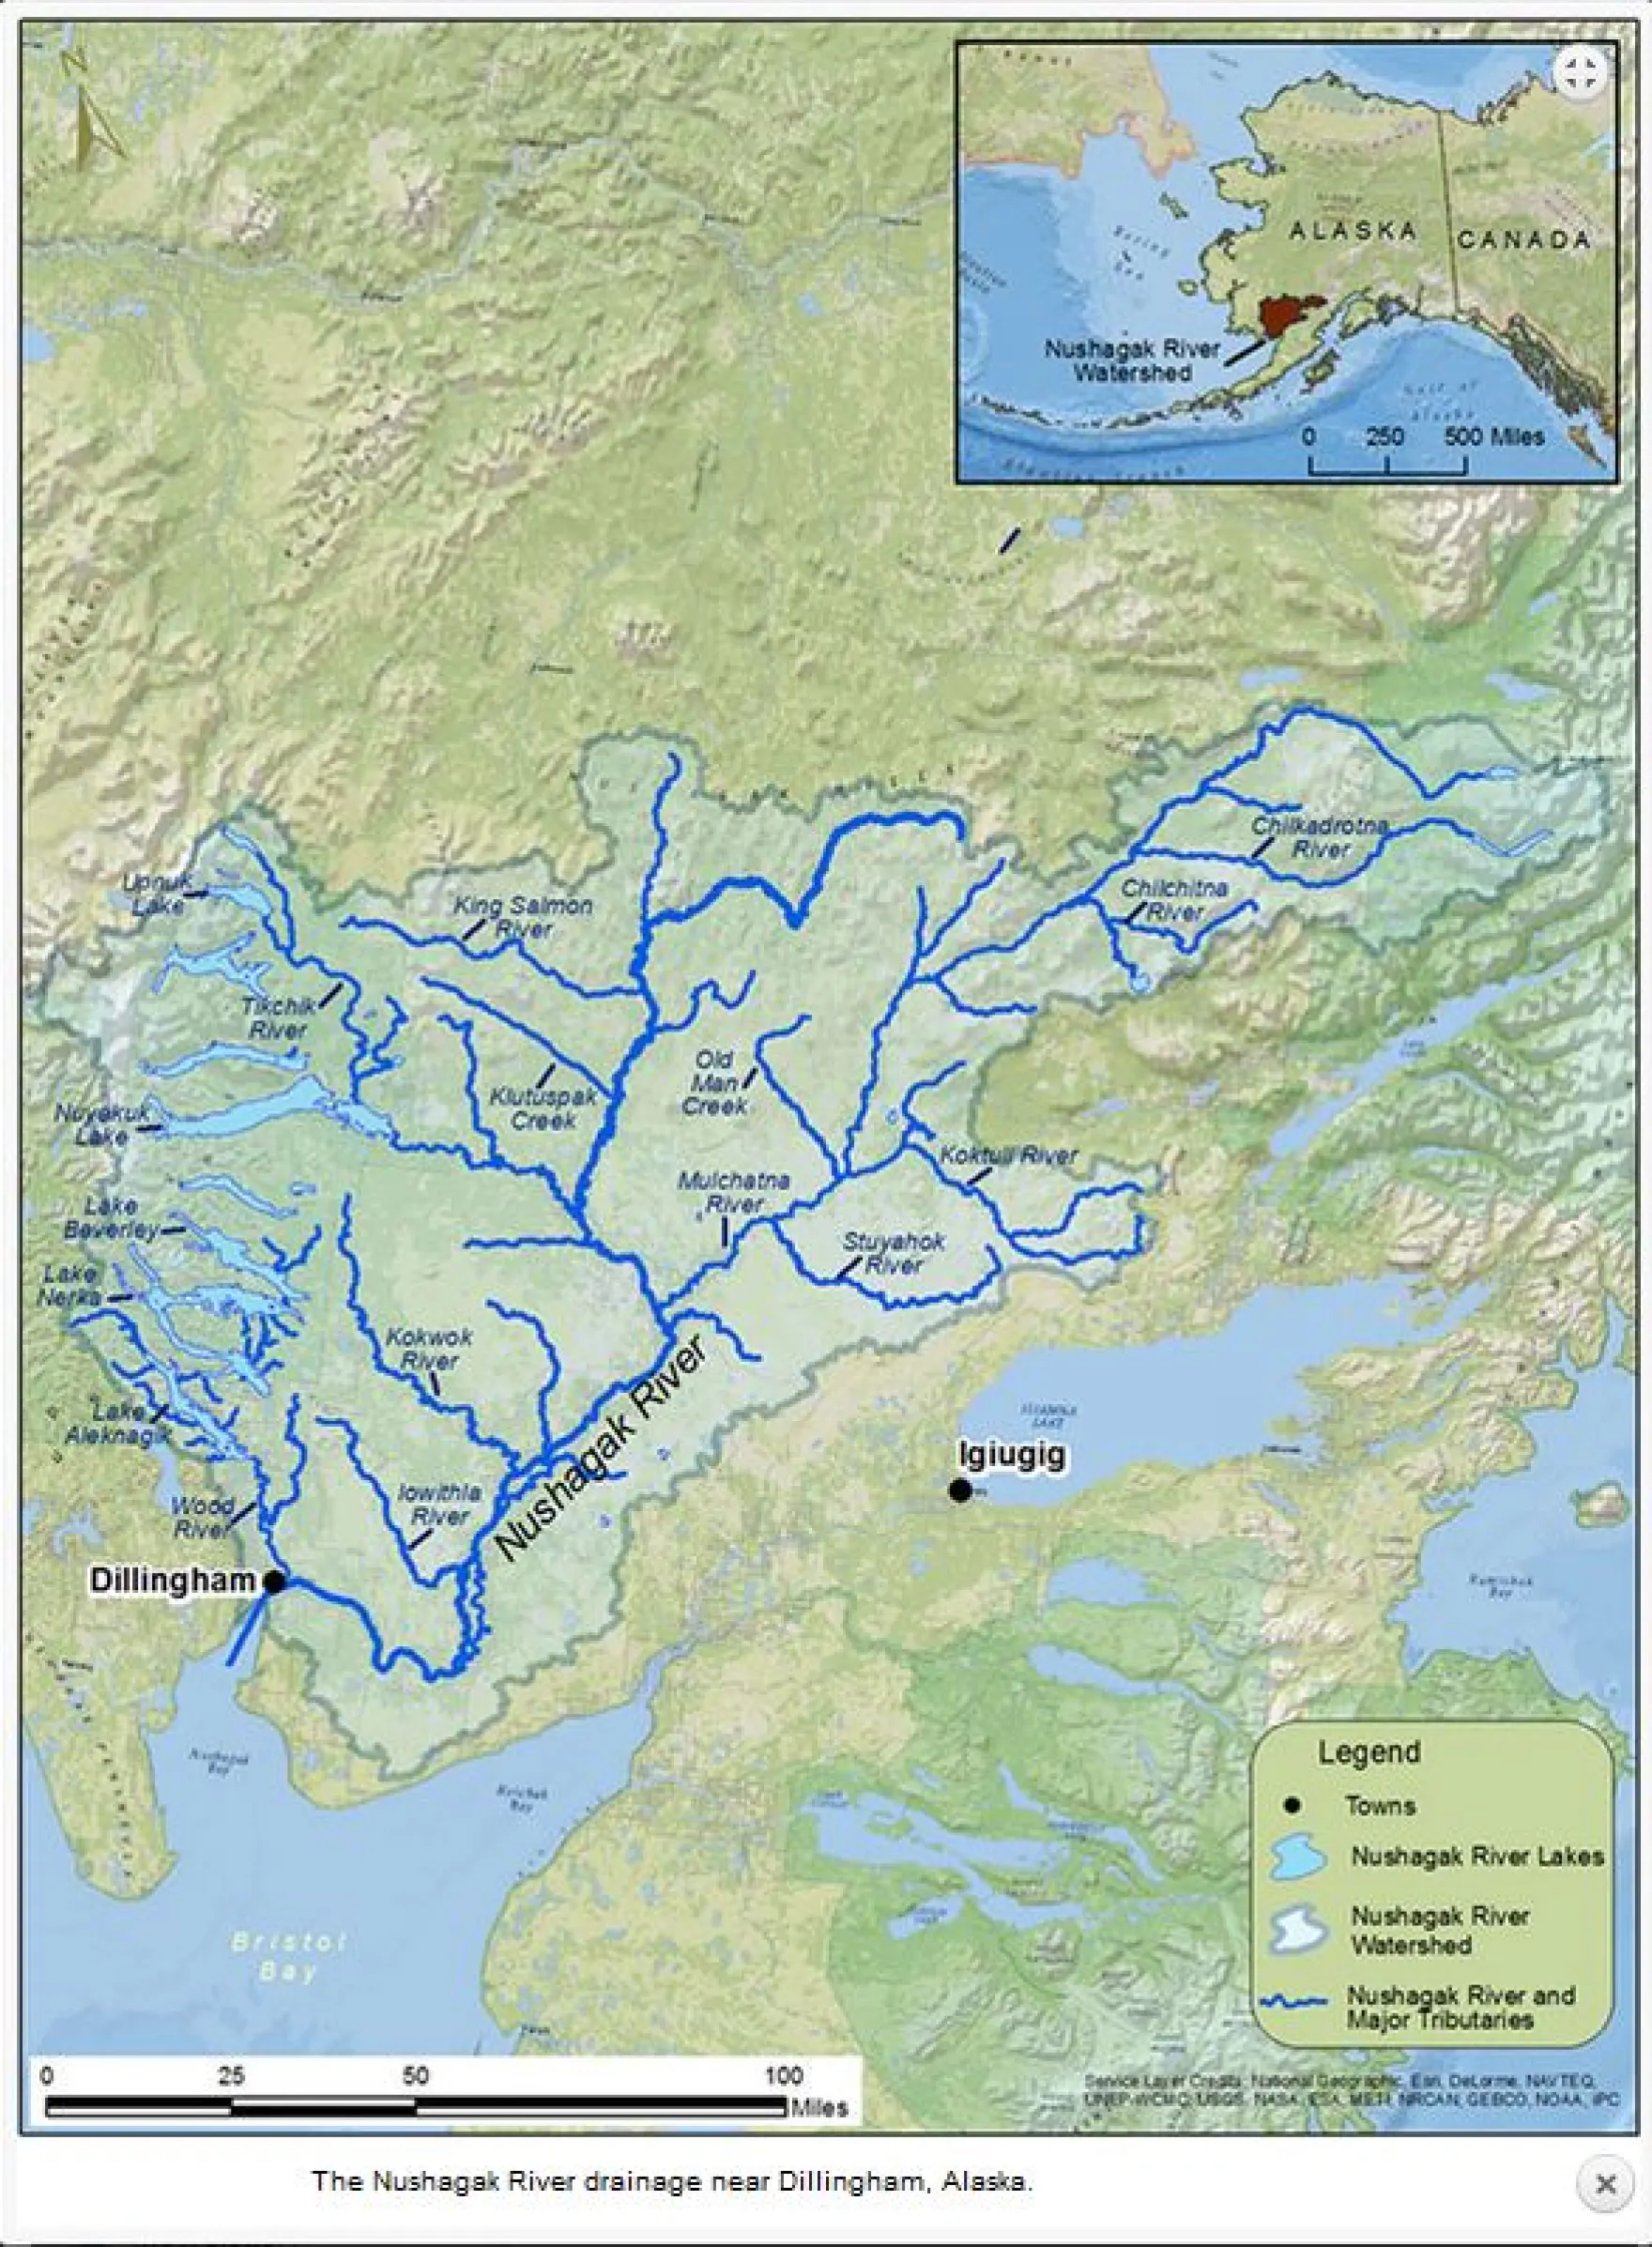
\includegraphics[width=0.6\linewidth,height=\textheight,keepaspectratio]{images/adfg_nushagak_watershed_map.png}

}

\caption{Nushagak River watershed and tributary map. Credit: Alaska
Department of Fish and Game.}

\end{figure}%

\section*{Overview}\label{overview}
\addcontentsline{toc}{section}{Overview}

\markright{Overview}

This document synthesizes existing water quality data for the Nushagak
River watershed (HUC6: 190303) in southwestern Alaska. The watershed
supports one of the world's most significant wild salmon fisheries and
is central to the cultural and subsistence economies of communities in
the region including Ekwok, New Koliganek, and New Stuyahok.

The analysis aggregates publicly available monitoring data from the EPA
Water Quality Portal (WQP) and USGS National Water Information System
(NWIS), supplemented by regulatory and scientific literature. The goal
is to establish an understanding of existing water quality conditions
across the Nushagak drainage and to identify data gaps where new
collaborative monitoring efforts could provide the greatest value.

\section*{Structure}\label{structure}
\addcontentsline{toc}{section}{Structure}

\markright{Structure}

The document is organized in three parts:

\textbf{Part I} assembles existing data sources, maps monitoring station
coverage, and catalogs what water quality parameters have been measured
historically.

\textbf{Part II} synthesizes key physical, chemical, and biological
parameters to characterize baseline conditions: temperature, pH,
dissolved oxygen, metals, nutrients, and their relevance to salmon
ecology.

\textbf{Part III} contextualizes this baseline within the RFP's two core
goals: establishing continuous monitoring efforts and enhancing data
management systems for the participating tribes.

\section*{Scope and Limitations}\label{scope-and-limitations}
\addcontentsline{toc}{section}{Scope and Limitations}

\markright{Scope and Limitations}

This synthesis covers the four HUC8 sub-basins of the Nushagak drainage:

\begin{itemize}
\tightlist
\item
  \textbf{19030301} --- Upper Nushagak River
\item
  \textbf{19030302} --- Mulchatna River
\item
  \textbf{19030303} --- Main Nushagak River
\item
  \textbf{19030304} --- Wood River
\end{itemize}

(See \url{https://water.usgs.gov/themes/hydrologic-units/} for visual
details).

All data presented derives from public repositories (WQP, NWIS) and
published literature. Data completeness varies by location and
parameter; gaps are noted throughout. This analysis is current as of
March 2024 for WQP/NWIS data.

\textbf{Prepared}: October 2026\\
\textbf{Data current through}: March 2024

\emph{AI Disclosure: We used Posit Assistant (Claude Haiku 4.5 and Qwen3
30B) to aid in debugging and deployment of this web report. All content
related to water quality was generated by Benjamin Meyer.}

\part{Part I: Watershed Context \& Existing Baseline}

\chapter{Watershed Overview}\label{watershed-overview}

\section{The Nushagak Drainage}\label{the-nushagak-drainage}

The Nushagak River extends more than 280 miles from the Alaska Range to
Bristol Bay, draining approximately 13,400 square miles of southwestern
Alaska. The watershed supports fisheries integral to the subsistence,
cultural, and economic well-being of the communities in the region.

\section{Participating Communities}\label{participating-communities}

Three tribes are proposing the collaborative monitoring effort:

\begin{itemize}
\tightlist
\item
  \textbf{Native Village of Ekwok}: Located on the Nushagak River
  mainstem
\item
  \textbf{New Koliganek Village Council}: Located at the Koliganek River
  confluence
\item
  \textbf{New Stuyahok Village Council}: Located on the Mulchatna River
\end{itemize}

Each community depends on wild salmon runs, and has a direct interest in
water quality conditions affecting fishery productivity and food safety.

\section{Why Monitor Water Quality}\label{why-monitor-water-quality}

Much as a physician may make health recommendations based on blood test
results, fishery managers may make recommendations for healthy
watersheds based on water quality data. Water quality parameters such as
temperature, pH, dissolved oxygen, nutrient levels, and contaminant
concentrations affect fish survival, growth, and reproduction. Baseline
monitoring allows communities to detect changes over time and to make
informed management decisions. Collaborative monitoring builds local
capacity and ensures that data collected reflects community-defined
priorities.

\section{Objectives of This Analysis}\label{objectives-of-this-analysis}

This document provides:

\begin{enumerate}
\def\labelenumi{\arabic{enumi}.}
\tightlist
\item
  An inventory of existing water quality data across the Nushagak
  drainage
\item
  A spatial and temporal summary of what has been measured and where
\item
  A characterization of baseline conditions for key parameters
\item
  Identification of gaps where new monitoring efforts would be most
  valuable
\item
  Context for designing monitoring strategies that align with the RFP's
  goals
\end{enumerate}

\emph{Chapters that follow explore each of these objectives in detail.}

\chapter{Data Sources and Inventory}\label{data-sources-and-inventory}

\section{Public Data Repositories}\label{public-data-repositories}

\subsection{Water Quality Portal (WQP)}\label{water-quality-portal-wqp}

The EPA Water Quality Portal (WQP) aggregates water quality data from
multiple sources: EPA's Storage and Retrieval (STORET) system, USGS
National Water Information System (NWIS), and state environmental agency
databases. For the Nushagak watershed, WQP contains physical and
chemical measurements (pH, temperature, conductivity, turbidity),
nutrients (nitrogen, phosphorus), trace metals, and biological
observations.

\textbf{Access}: Queried via the \texttt{dataRetrieval} R package using
HUC identifiers. Data are current through March 2024.

\subsection{USGS National Water Information System
(NWIS)}\label{usgs-national-water-information-system-nwis}

NWIS contains streamflow measurements, continuous water temperature
records from deployed sensors, and periodic water chemistry samples
collected by USGS. These data often span decades and provide context for
long-term trends.

\textbf{Access}: Queried via \texttt{dataRetrieval::readNWISdata()} in R
scripts. Site identifiers are referenced in WQP but can also be accessed
directly.

\subsection{Alaska Department of Environmental Conservation (DEC) Water
Quality
Portal}\label{alaska-department-of-environmental-conservation-dec-water-quality-portal}

Alaska DEC maintains ambient water quality monitoring data, Section
303(d) impairment assessments, and reports on grant-funded monitoring
projects. Coverage of the Nushagak drainage is variable.

\textbf{Access}: Manual browsing of the DEC portal
(https://dec.alaska.gov/water/) or direct contact with DEC regional
offices for data export.

\begin{center}\rule{0.5\linewidth}{0.5pt}\end{center}

\section{Secondary Literature and Regulatory
Data}\label{secondary-literature-and-regulatory-data}

\subsection{EPA Bristol Bay Watershed
Assessment}\label{epa-bristol-bay-watershed-assessment}

The EPA's \href{https://www.epa.gov/bristolbay}{Bristol Bay Watershed
Assessment} synthesizes data on aquatic ecosystems, fisheries, and water
quality across the Bristol Bay region, including the Nushagak drainage.
Published reports include summary tables of trace metal concentrations
and baseline conditions for comparison.

\textbf{Access}: Published reports; data presented in tables and
narrative form.

\subsection{Pebble Project Environmental Baseline
Document}\label{pebble-project-environmental-baseline-document}

The Pebble Project Environmental Impact Statement included extensive
baseline water quality monitoring in the Mulchatna and Koktuli river
drainages (tributaries of the Nushagak). These data include surface
water chemistry, dissolved and total metals, alkalinity, and stream
temperature records.

\textbf{Access}: Available through the Pebble Project EIS website; data
in PDF tables (may require OCR or manual extraction).

\subsection{Academic and Tribal
Monitoring}\label{academic-and-tribal-monitoring}

Cook Inletkeeper, Bristol Bay Native Association (BBNA), and academic
researchers have collected water quality and stream temperature data
relevant to the watershed. Some data are publicly available
(e.g.~\href{https://aktemp.uaa.alaska.edu/\#/}{AKTEMP}); others are held
by tribal organizations or require partnership agreements.

\textbf{Access}: Variable; direct contact with organizations recommended
(e.g.~University of Washington Alaska Salmon Program)

\begin{center}\rule{0.5\linewidth}{0.5pt}\end{center}

\section{Data Compilation Strategy}\label{data-compilation-strategy}

This analysis prioritizes directly queryable data (WQP, NWIS) to ensure
reproducibility and transparency. Grey literature is referenced to
contextualize findings and identify historical patterns, but analysis
for now focuses on accessible, reproducible data pipelines.

\subsection{Data Quality and
Validation}\label{data-quality-and-validation}

WQP data are submitted by multiple organizations using the EPA's Water
Quality eXchange (WQX) standard, but data entry practices and metadata
quality vary.

For future work or larger-scale data integration, the EPA's
\textbf{Tools for Automated Data Analysis (TADA)} framework provides a
systematic approach to data discovery, validation, and cleaning. TADA
includes automated quality control screens, detection limit handling,
unit harmonization, and flagging of invalid metadata using EPA's WQX
domain validation services. Organizations preparing data submissions to
WQP can use TADA to ensure consistency before archival. See the Data
Management chapter for a discussion of TADA's role in the proposed
monitoring system.

A summary of stations and observation counts by HUC follows in the next
chapter.

\chapter{Spatial Coverage of Monitoring
Stations}\label{spatial-coverage-of-monitoring-stations}

\begin{Shaded}
\begin{Highlighting}[]
\FunctionTok{library}\NormalTok{(dataRetrieval)}
\FunctionTok{library}\NormalTok{(dplyr)}
\FunctionTok{library}\NormalTok{(sf)}
\FunctionTok{library}\NormalTok{(leaflet)}
\FunctionTok{library}\NormalTok{(ggplot2)}

\CommentTok{\# Four HUC8s draining into the Nushagak River. HUC8 19030305 (Togiak River)}
\CommentTok{\# drains separately into Bristol Bay and is excluded; see Observations below.}
\NormalTok{nushagak\_hucs }\OtherTok{\textless{}{-}} \FunctionTok{c}\NormalTok{(}\StringTok{"19030301"}\NormalTok{, }\StringTok{"19030302"}\NormalTok{, }\StringTok{"19030303"}\NormalTok{, }\StringTok{"19030304"}\NormalTok{)}

\CommentTok{\# Fetch station inventory}
\FunctionTok{message}\NormalTok{(}\StringTok{"Querying WQP for the four Nushagak HUC8 sub{-}basins..."}\NormalTok{)}
\NormalTok{wq\_inventory }\OtherTok{\textless{}{-}} \FunctionTok{data.frame}\NormalTok{()}

\ControlFlowTok{for}\NormalTok{ (huc }\ControlFlowTok{in}\NormalTok{ nushagak\_hucs) \{}
\NormalTok{  temp }\OtherTok{\textless{}{-}} \FunctionTok{whatWQPdata}\NormalTok{(}\AttributeTok{huc =}\NormalTok{ huc)}
\NormalTok{  temp}\SpecialCharTok{$}\NormalTok{HUC }\OtherTok{\textless{}{-}}\NormalTok{ huc}
\NormalTok{  wq\_inventory }\OtherTok{\textless{}{-}} \FunctionTok{rbind}\NormalTok{(wq\_inventory, temp)}
\NormalTok{\}}

\CommentTok{\# Convert to spatial object}
\NormalTok{wq\_sf }\OtherTok{\textless{}{-}}\NormalTok{ wq\_inventory }\SpecialCharTok{\%\textgreater{}\%}
  \FunctionTok{filter}\NormalTok{(}\SpecialCharTok{!}\FunctionTok{is.na}\NormalTok{(lon), }\SpecialCharTok{!}\FunctionTok{is.na}\NormalTok{(lat)) }\SpecialCharTok{\%\textgreater{}\%}
  \FunctionTok{st\_as\_sf}\NormalTok{(}\AttributeTok{coords =} \FunctionTok{c}\NormalTok{(}\StringTok{"lon"}\NormalTok{, }\StringTok{"lat"}\NormalTok{), }\AttributeTok{crs =} \DecValTok{4326}\NormalTok{)}
\end{Highlighting}
\end{Shaded}

\section{Overview}\label{overview-1}

Monitoring stations in the Nushagak drainage are distributed across
streams and lakes in four HUC8 sub-basins. The map below displays all
stations with water quality data available in the WQP.

\begin{Shaded}
\begin{Highlighting}[]
\FunctionTok{leaflet}\NormalTok{(wq\_sf) }\SpecialCharTok{\%\textgreater{}\%}
  \FunctionTok{addProviderTiles}\NormalTok{(providers}\SpecialCharTok{$}\NormalTok{Esri.WorldTopoMap, }\AttributeTok{group =} \StringTok{"Topo"}\NormalTok{) }\SpecialCharTok{\%\textgreater{}\%}
  \FunctionTok{addProviderTiles}\NormalTok{(providers}\SpecialCharTok{$}\NormalTok{Esri.WorldImagery, }\AttributeTok{group =} \StringTok{"Satellite"}\NormalTok{) }\SpecialCharTok{\%\textgreater{}\%}
  \FunctionTok{addCircleMarkers}\NormalTok{(}
    \AttributeTok{radius =} \DecValTok{6}\NormalTok{,}
    \AttributeTok{color =} \StringTok{"\#0072B2"}\NormalTok{,}
    \AttributeTok{weight =} \DecValTok{1}\NormalTok{,}
    \AttributeTok{fillOpacity =} \FloatTok{0.7}\NormalTok{,}
    \AttributeTok{popup =} \SpecialCharTok{\textasciitilde{}}\FunctionTok{paste0}\NormalTok{(}
      \StringTok{"\textless{}b\textgreater{}"}\NormalTok{, MonitoringLocationName, }\StringTok{"\textless{}/b\textgreater{}\textless{}br\textgreater{}"}\NormalTok{,}
      \StringTok{"ID: "}\NormalTok{, MonitoringLocationIdentifier, }\StringTok{"\textless{}br\textgreater{}"}\NormalTok{,}
      \StringTok{"Org: "}\NormalTok{, OrganizationFormalName, }\StringTok{"\textless{}br\textgreater{}"}\NormalTok{,}
      \StringTok{"Results: "}\NormalTok{, resultCount}
\NormalTok{    ),}
    \AttributeTok{clusterOptions =} \FunctionTok{markerClusterOptions}\NormalTok{()}
\NormalTok{  ) }\SpecialCharTok{\%\textgreater{}\%}
  \FunctionTok{addLayersControl}\NormalTok{(}
    \AttributeTok{baseGroups =} \FunctionTok{c}\NormalTok{(}\StringTok{"Topo"}\NormalTok{, }\StringTok{"Satellite"}\NormalTok{),}
    \AttributeTok{options =} \FunctionTok{layersControlOptions}\NormalTok{(}\AttributeTok{collapsed =} \ConstantTok{FALSE}\NormalTok{)}
\NormalTok{  )}
\end{Highlighting}
\end{Shaded}

\section{Summary by HUC}\label{summary-by-huc}

\begin{Shaded}
\begin{Highlighting}[]
\NormalTok{huc\_summary }\OtherTok{\textless{}{-}}\NormalTok{ wq\_inventory }\SpecialCharTok{\%\textgreater{}\%}
  \FunctionTok{group\_by}\NormalTok{(HUC) }\SpecialCharTok{\%\textgreater{}\%}
  \FunctionTok{summarize}\NormalTok{(}
    \AttributeTok{Stations =} \FunctionTok{n\_distinct}\NormalTok{(MonitoringLocationIdentifier),}
    \AttributeTok{Total\_Results =} \FunctionTok{sum}\NormalTok{(resultCount, }\AttributeTok{na.rm =} \ConstantTok{TRUE}\NormalTok{),}
    \AttributeTok{Organizations =} \FunctionTok{n\_distinct}\NormalTok{(OrganizationFormalName),}
    \AttributeTok{.groups =} \StringTok{"drop"}
\NormalTok{  ) }\SpecialCharTok{\%\textgreater{}\%}
  \FunctionTok{arrange}\NormalTok{(HUC) }\SpecialCharTok{\%\textgreater{}\%}
  \FunctionTok{mutate}\NormalTok{(}
    \AttributeTok{HUC\_Name =} \FunctionTok{case\_when}\NormalTok{(}
\NormalTok{      HUC }\SpecialCharTok{==} \StringTok{"19030301"} \SpecialCharTok{\textasciitilde{}} \StringTok{"Upper Nushagak"}\NormalTok{,}
\NormalTok{      HUC }\SpecialCharTok{==} \StringTok{"19030302"} \SpecialCharTok{\textasciitilde{}} \StringTok{"Mulchatna"}\NormalTok{,}
\NormalTok{      HUC }\SpecialCharTok{==} \StringTok{"19030303"} \SpecialCharTok{\textasciitilde{}} \StringTok{"Main Nushagak"}\NormalTok{,}
\NormalTok{      HUC }\SpecialCharTok{==} \StringTok{"19030304"} \SpecialCharTok{\textasciitilde{}} \StringTok{"Wood"}\NormalTok{,}
      \ConstantTok{TRUE} \SpecialCharTok{\textasciitilde{}}\NormalTok{ HUC}
\NormalTok{    )}
\NormalTok{  ) }\SpecialCharTok{\%\textgreater{}\%}
  \FunctionTok{select}\NormalTok{(HUC, HUC\_Name, Stations, Total\_Results, Organizations) }\SpecialCharTok{\%\textgreater{}\%}
  \FunctionTok{rename}\NormalTok{(}\StringTok{"Sub{-}basin"} \OtherTok{=}\NormalTok{ HUC\_Name, }\StringTok{"Monitoring Locations"} \OtherTok{=}\NormalTok{ Stations, }\StringTok{"Total Observations"} \OtherTok{=}\NormalTok{ Total\_Results, }\StringTok{"Data Providers"} \OtherTok{=}\NormalTok{ Organizations)}

\NormalTok{knitr}\SpecialCharTok{::}\FunctionTok{kable}\NormalTok{(huc\_summary, }\AttributeTok{caption =} \StringTok{"Monitoring Coverage by HUC8 Sub{-}basin"}\NormalTok{)}
\end{Highlighting}
\end{Shaded}

\begin{longtable}[]{@{}
  >{\raggedright\arraybackslash}p{(\linewidth - 8\tabcolsep) * \real{0.1139}}
  >{\raggedright\arraybackslash}p{(\linewidth - 8\tabcolsep) * \real{0.1899}}
  >{\raggedleft\arraybackslash}p{(\linewidth - 8\tabcolsep) * \real{0.2658}}
  >{\raggedleft\arraybackslash}p{(\linewidth - 8\tabcolsep) * \real{0.2405}}
  >{\raggedleft\arraybackslash}p{(\linewidth - 8\tabcolsep) * \real{0.1899}}@{}}
\caption{Monitoring Coverage by HUC8 Sub-basin}\tabularnewline
\toprule\noalign{}
\begin{minipage}[b]{\linewidth}\raggedright
HUC
\end{minipage} & \begin{minipage}[b]{\linewidth}\raggedright
Sub-basin
\end{minipage} & \begin{minipage}[b]{\linewidth}\raggedleft
Monitoring Locations
\end{minipage} & \begin{minipage}[b]{\linewidth}\raggedleft
Total Observations
\end{minipage} & \begin{minipage}[b]{\linewidth}\raggedleft
Data Providers
\end{minipage} \\
\midrule\noalign{}
\endfirsthead
\toprule\noalign{}
\begin{minipage}[b]{\linewidth}\raggedright
HUC
\end{minipage} & \begin{minipage}[b]{\linewidth}\raggedright
Sub-basin
\end{minipage} & \begin{minipage}[b]{\linewidth}\raggedleft
Monitoring Locations
\end{minipage} & \begin{minipage}[b]{\linewidth}\raggedleft
Total Observations
\end{minipage} & \begin{minipage}[b]{\linewidth}\raggedleft
Data Providers
\end{minipage} \\
\midrule\noalign{}
\endhead
\bottomrule\noalign{}
\endlastfoot
19030301 & Upper Nushagak & 20 & 1324 & 3 \\
19030302 & Mulchatna & 135 & 8311 & 3 \\
19030303 & Main Nushagak & 221 & 6051 & 3 \\
19030304 & Wood & 42 & 446 & 1 \\
\end{longtable}

\section{Data Provider Distribution}\label{data-provider-distribution}

\begin{Shaded}
\begin{Highlighting}[]
\NormalTok{provider\_summary }\OtherTok{\textless{}{-}}\NormalTok{ wq\_inventory }\SpecialCharTok{\%\textgreater{}\%}
  \FunctionTok{group\_by}\NormalTok{(OrganizationFormalName) }\SpecialCharTok{\%\textgreater{}\%}
  \FunctionTok{summarize}\NormalTok{(}
    \AttributeTok{Stations =} \FunctionTok{n\_distinct}\NormalTok{(MonitoringLocationIdentifier),}
    \AttributeTok{Total\_Results =} \FunctionTok{sum}\NormalTok{(resultCount, }\AttributeTok{na.rm =} \ConstantTok{TRUE}\NormalTok{),}
    \AttributeTok{.groups =} \StringTok{"drop"}
\NormalTok{  ) }\SpecialCharTok{\%\textgreater{}\%}
  \FunctionTok{arrange}\NormalTok{(}\FunctionTok{desc}\NormalTok{(Total\_Results)) }\SpecialCharTok{\%\textgreater{}\%}
  \FunctionTok{rename}\NormalTok{(}\StringTok{"Organization"} \OtherTok{=}\NormalTok{ OrganizationFormalName, }\StringTok{"Stations"} \OtherTok{=}\NormalTok{ Stations, }\StringTok{"Observations"} \OtherTok{=}\NormalTok{ Total\_Results)}

\NormalTok{knitr}\SpecialCharTok{::}\FunctionTok{kable}\NormalTok{(provider\_summary, }\AttributeTok{caption =} \StringTok{"Data Contributions by Organization"}\NormalTok{)}
\end{Highlighting}
\end{Shaded}

\begin{longtable}[]{@{}
  >{\raggedright\arraybackslash}p{(\linewidth - 4\tabcolsep) * \real{0.7250}}
  >{\raggedleft\arraybackslash}p{(\linewidth - 4\tabcolsep) * \real{0.1125}}
  >{\raggedleft\arraybackslash}p{(\linewidth - 4\tabcolsep) * \real{0.1625}}@{}}
\caption{Data Contributions by Organization}\tabularnewline
\toprule\noalign{}
\begin{minipage}[b]{\linewidth}\raggedright
Organization
\end{minipage} & \begin{minipage}[b]{\linewidth}\raggedleft
Stations
\end{minipage} & \begin{minipage}[b]{\linewidth}\raggedleft
Observations
\end{minipage} \\
\midrule\noalign{}
\endfirsthead
\toprule\noalign{}
\begin{minipage}[b]{\linewidth}\raggedright
Organization
\end{minipage} & \begin{minipage}[b]{\linewidth}\raggedleft
Stations
\end{minipage} & \begin{minipage}[b]{\linewidth}\raggedleft
Observations
\end{minipage} \\
\midrule\noalign{}
\endhead
\bottomrule\noalign{}
\endlastfoot
USGS Alaska Water Science Center & 228 & 7463 \\
National Park Service Water Resources Division & 104 & 5157 \\
Alaska Dept of Environmental Conservation - Water Quality & 50 & 2523 \\
Alaska Soil and Water Conservation District & 36 & 989 \\
\end{longtable}

\section{Observations}\label{observations}

The coverage varies by sub-basin, with the Upper Nushagak (19030301) and
main Nushagak system (19030303) having the most monitoring
infrastructure. The Mulchatna (19030302) has moderate coverage, while
the Wood River drainage (19030304) has fewer established stations. This
distribution reflects historical research emphasis and the availability
of USGS gaging stations. (Note: HUC8 19030305, which comprises the
Togiak River system, is excluded from this analysis as it drains
separately into Bristol Bay rather than the Nushagak River.)

USGS contributes the majority of observations, reflecting the long-term
nature of federal streamflow and water chemistry monitoring. Tribal and
state efforts are also evident and represent valuable local capacity.

\textbf{Data Quality Note}: The WQP station inventory includes
approximately 212 stations across the Nushagak HUCs that are registered
in the system but show zero water quality results in the current API
response. These may represent monitoring locations where data collection
has occurred but results are not yet integrated into the WQP database,
or where records exist in alternate formats. These sites are included in
the station count above but do not contribute to the observation totals.

\begin{center}\rule{0.5\linewidth}{0.5pt}\end{center}

The next chapter examines what water quality parameters have been
measured and identifies temporal and spatial gaps in the existing data.

\chapter{Water Quality Parameters: Inventory and
Gaps}\label{water-quality-parameters-inventory-and-gaps}

\begin{Shaded}
\begin{Highlighting}[]
\FunctionTok{library}\NormalTok{(dataRetrieval)}
\FunctionTok{library}\NormalTok{(dplyr)}
\FunctionTok{library}\NormalTok{(ggplot2)}

\CommentTok{\# Fetch parameter data for all five HUCs}
\NormalTok{nushagak\_hucs }\OtherTok{\textless{}{-}} \FunctionTok{c}\NormalTok{(}\StringTok{"19030301"}\NormalTok{, }\StringTok{"19030302"}\NormalTok{, }\StringTok{"19030303"}\NormalTok{, }\StringTok{"19030304"}\NormalTok{)}

\FunctionTok{message}\NormalTok{(}\StringTok{"Querying WQP for parameter observations..."}\NormalTok{)}
\NormalTok{wq\_data }\OtherTok{\textless{}{-}} \FunctionTok{data.frame}\NormalTok{()}

\ControlFlowTok{for}\NormalTok{ (huc }\ControlFlowTok{in}\NormalTok{ nushagak\_hucs) \{}
\NormalTok{  temp }\OtherTok{\textless{}{-}} \FunctionTok{readWQPdata}\NormalTok{(}\AttributeTok{huc =}\NormalTok{ huc, }\AttributeTok{sampleMedia =} \StringTok{"Water"}\NormalTok{)}
\NormalTok{  temp}\SpecialCharTok{$}\NormalTok{HUC }\OtherTok{\textless{}{-}}\NormalTok{ huc}
\NormalTok{  wq\_data }\OtherTok{\textless{}{-}} \FunctionTok{rbind}\NormalTok{(wq\_data, temp)}
\NormalTok{\}}

\CommentTok{\# Remove duplicates and NA characteristic names}
\NormalTok{wq\_data }\OtherTok{\textless{}{-}}\NormalTok{ wq\_data }\SpecialCharTok{\%\textgreater{}\%}
  \FunctionTok{filter}\NormalTok{(}\SpecialCharTok{!}\FunctionTok{is.na}\NormalTok{(CharacteristicName))}
\end{Highlighting}
\end{Shaded}

\section{Parameter Frequency}\label{parameter-frequency}

The following parameters have been measured in the Nushagak watershed:

\begin{Shaded}
\begin{Highlighting}[]
\NormalTok{param\_freq }\OtherTok{\textless{}{-}}\NormalTok{ wq\_data }\SpecialCharTok{\%\textgreater{}\%}
  \FunctionTok{group\_by}\NormalTok{(CharacteristicName) }\SpecialCharTok{\%\textgreater{}\%}
  \FunctionTok{summarize}\NormalTok{(}
    \AttributeTok{Observations =} \FunctionTok{n}\NormalTok{(),}
    \AttributeTok{Stations =} \FunctionTok{n\_distinct}\NormalTok{(MonitoringLocationIdentifier),}
    \AttributeTok{.groups =} \StringTok{"drop"}
\NormalTok{  ) }\SpecialCharTok{\%\textgreater{}\%}
  \FunctionTok{arrange}\NormalTok{(}\FunctionTok{desc}\NormalTok{(Observations)) }\SpecialCharTok{\%\textgreater{}\%}
  \FunctionTok{rename}\NormalTok{(}\StringTok{"Parameter"} \OtherTok{=}\NormalTok{ CharacteristicName, }\StringTok{"Measurements"} \OtherTok{=}\NormalTok{ Observations, }\StringTok{"Unique Stations"} \OtherTok{=}\NormalTok{ Stations)}

\CommentTok{\# Display top 20 parameters}
\NormalTok{knitr}\SpecialCharTok{::}\FunctionTok{kable}\NormalTok{(}
  \FunctionTok{head}\NormalTok{(param\_freq, }\DecValTok{20}\NormalTok{),}
  \AttributeTok{caption =} \StringTok{"Most Frequently Measured Water Quality Parameters (Top 20)"}
\NormalTok{)}
\end{Highlighting}
\end{Shaded}

\begin{longtable}[]{@{}lrr@{}}
\caption{Most Frequently Measured Water Quality Parameters (Top
20)}\tabularnewline
\toprule\noalign{}
Parameter & Measurements & Unique Stations \\
\midrule\noalign{}
\endfirsthead
\toprule\noalign{}
Parameter & Measurements & Unique Stations \\
\midrule\noalign{}
\endhead
\bottomrule\noalign{}
\endlastfoot
Stream flow, instantaneous & 940 & 10 \\
Temperature, water & 902 & 196 \\
Specific conductance & 488 & 197 \\
Stream width measure & 452 & 21 \\
pH & 446 & 196 \\
Temperature, air & 335 & 19 \\
Height, gage & 306 & 13 \\
Oxygen & 268 & 1 \\
Total dissolved solids & 259 & 14 \\
Acidity, (H+) & 207 & 22 \\
Iron & 205 & 53 \\
Barometric pressure & 173 & 47 \\
Manganese & 172 & 53 \\
Turbidity & 170 & 50 \\
Calcium & 163 & 53 \\
Magnesium & 163 & 53 \\
Sodium & 163 & 53 \\
Potassium & 161 & 53 \\
Uranium & 154 & 129 \\
Depth & 146 & 26 \\
\end{longtable}

\section{Key Parameter Categories}\label{key-parameter-categories}

\subsection{Physical Properties}\label{physical-properties}

\begin{itemize}
\tightlist
\item
  \textbf{Temperature}: Essential for salmon habitat assessment;
  continuous monitoring data available from USGS gages
\item
  \textbf{Conductivity \& Specific Conductance}: Indicates
  mineralization and ionic composition
\item
  \textbf{Turbidity}: Affects light penetration; high values can
  indicate erosion or glacial discharge
\end{itemize}

\subsection{Chemical Properties}\label{chemical-properties}

\begin{itemize}
\tightlist
\item
  \textbf{pH}: Affects aquatic chemistry and organism physiology
\item
  \textbf{Dissolved Oxygen}: Critical for salmonid survival; cold,
  well-oxygenated water preferred
\item
  \textbf{Alkalinity \& Hardness}: Buffer capacity against acid inputs
\end{itemize}

\subsection{Nutrients}\label{nutrients}

\begin{itemize}
\tightlist
\item
  \textbf{Nitrogen (various forms)}: Nitrate, nitrite, ammonia, total
  nitrogen
\item
  \textbf{Phosphorus (various forms)}: Orthophosphate, total phosphorus
\item
  (Limited frequency in existing data; opportunity for expanded
  monitoring)
\end{itemize}

\subsection{Trace Elements \& Metals}\label{trace-elements-metals}

\begin{itemize}
\tightlist
\item
  \textbf{Copper}: Abnormal levels can be toxic to aquatic life;
  relevant to mining activity concerns
\item
  \textbf{Zinc, Lead, Cadmium, Chromium}: Other metals detected;
  relevance context-dependent
\item
  \textbf{Molybdenum}: Associated with geochemistry and mining scenarios
\end{itemize}

\subsection{Biological}\label{biological}

\begin{itemize}
\tightlist
\item
  \textbf{Algal and macroinvertebrate sampling}: Limited in frequency;
  primarily USGS and academic efforts
\end{itemize}

\begin{center}\rule{0.5\linewidth}{0.5pt}\end{center}

\section{Data Gaps and Monitoring
Opportunities}\label{data-gaps-and-monitoring-opportunities}

Based on the inventory, the following represent priorities for expanded
collaborative monitoring:

\begin{enumerate}
\def\labelenumi{\arabic{enumi}.}
\item
  \textbf{Continuous Temperature Data}: Few sites have high-frequency
  temperature loggers; salmon thermal habitat monitoring would benefit
  from denser deployment.
\item
  \textbf{Nutrients (N, P)}: Few measurements in existing WQP data;
  baseline nutrient levels are poorly characterized across most of the
  watershed.
\item
  \textbf{Spatial Coverage in Wood River and Nuyakuk Drainages}: Fewer
  historical stations in these sub-basins; new effort could establish
  baseline for comparison.
\item
  \textbf{Biological Metrics}: Macroinvertebrate and periphyton sampling
  is limited. Fish presence/absence and juvenile salmon surveys would
  complement chemistry data.
\item
  \textbf{Seasonal and High-Flow Sampling}: Most data are episodic;
  systematic seasonal sampling would reveal temperature, discharge, and
  contaminant dynamics.
\end{enumerate}

\begin{center}\rule{0.5\linewidth}{0.5pt}\end{center}

These gaps inform the monitoring design recommendations in Part III.

\part{Part II: Baseline Water Quality Synthesis}

\chapter{Physical and Chemical
Baseline}\label{physical-and-chemical-baseline}

\begin{Shaded}
\begin{Highlighting}[]
\FunctionTok{library}\NormalTok{(dataRetrieval)}
\FunctionTok{library}\NormalTok{(dplyr)}
\FunctionTok{library}\NormalTok{(ggplot2)}

\CommentTok{\# Key parameters for physical/chemical baseline}
\NormalTok{key\_params }\OtherTok{\textless{}{-}} \FunctionTok{c}\NormalTok{(}\StringTok{"pH"}\NormalTok{, }\StringTok{"Temperature, water"}\NormalTok{, }\StringTok{"Dissolved oxygen (DO)"}\NormalTok{, }
                \StringTok{"Specific conductance"}\NormalTok{, }\StringTok{"Turbidity"}\NormalTok{)}

\NormalTok{nushagak\_hucs }\OtherTok{\textless{}{-}} \FunctionTok{c}\NormalTok{(}\StringTok{"19030301"}\NormalTok{, }\StringTok{"19030302"}\NormalTok{, }\StringTok{"19030303"}\NormalTok{, }\StringTok{"19030304"}\NormalTok{)}

\CommentTok{\# Fetch data for key parameters}
\FunctionTok{message}\NormalTok{(}\StringTok{"Querying WQP for key physical/chemical parameters..."}\NormalTok{)}
\NormalTok{wq\_data }\OtherTok{\textless{}{-}} \FunctionTok{readWQPdata}\NormalTok{(}\AttributeTok{huc =}\NormalTok{ nushagak\_hucs, }\AttributeTok{sampleMedia =} \StringTok{"Water"}\NormalTok{)}

\CommentTok{\# Filter to key parameters}
\NormalTok{wq\_key }\OtherTok{\textless{}{-}}\NormalTok{ wq\_data }\SpecialCharTok{\%\textgreater{}\%}
  \FunctionTok{filter}\NormalTok{(CharacteristicName }\SpecialCharTok{\%in\%}\NormalTok{ key\_params) }\SpecialCharTok{\%\textgreater{}\%}
  \FunctionTok{filter}\NormalTok{(}\SpecialCharTok{!}\FunctionTok{is.na}\NormalTok{(ResultMeasureValue))}
\end{Highlighting}
\end{Shaded}

\section{Temperature}\label{temperature}

Water temperature is fundamental to salmon ecology. Optimal ranges vary
by species and life stage, but most Pacific salmon prefer cool water
(≤16°C) and suffer stress at temperatures \textgreater20°C.

\begin{Shaded}
\begin{Highlighting}[]
\NormalTok{temp\_data }\OtherTok{\textless{}{-}}\NormalTok{ wq\_key }\SpecialCharTok{\%\textgreater{}\%}
  \FunctionTok{filter}\NormalTok{(CharacteristicName }\SpecialCharTok{==} \StringTok{"Temperature, water"}\NormalTok{) }\SpecialCharTok{\%\textgreater{}\%}
  \FunctionTok{select}\NormalTok{(ResultMeasureValue) }\SpecialCharTok{\%\textgreater{}\%}
  \FunctionTok{mutate}\NormalTok{(}\AttributeTok{Temperature\_C =} \FunctionTok{as.numeric}\NormalTok{(ResultMeasureValue)) }\SpecialCharTok{\%\textgreater{}\%}
  \FunctionTok{select}\NormalTok{(}\SpecialCharTok{{-}}\NormalTok{ResultMeasureValue)}

\ControlFlowTok{if}\NormalTok{ (}\FunctionTok{nrow}\NormalTok{(temp\_data) }\SpecialCharTok{\textgreater{}} \DecValTok{0}\NormalTok{) \{}
\NormalTok{  temp\_stats }\OtherTok{\textless{}{-}}\NormalTok{ temp\_data }\SpecialCharTok{\%\textgreater{}\%}
    \FunctionTok{summarize}\NormalTok{(}
      \AttributeTok{N =} \FunctionTok{n}\NormalTok{(),}
      \AttributeTok{Mean =} \FunctionTok{mean}\NormalTok{(Temperature\_C, }\AttributeTok{na.rm =} \ConstantTok{TRUE}\NormalTok{),}
      \AttributeTok{Median =} \FunctionTok{median}\NormalTok{(Temperature\_C, }\AttributeTok{na.rm =} \ConstantTok{TRUE}\NormalTok{),}
      \AttributeTok{Min =} \FunctionTok{min}\NormalTok{(Temperature\_C, }\AttributeTok{na.rm =} \ConstantTok{TRUE}\NormalTok{),}
      \AttributeTok{Max =} \FunctionTok{max}\NormalTok{(Temperature\_C, }\AttributeTok{na.rm =} \ConstantTok{TRUE}\NormalTok{),}
      \AttributeTok{SD =} \FunctionTok{sd}\NormalTok{(Temperature\_C, }\AttributeTok{na.rm =} \ConstantTok{TRUE}\NormalTok{)}
\NormalTok{    )}
  
\NormalTok{  knitr}\SpecialCharTok{::}\FunctionTok{kable}\NormalTok{(temp\_stats, }\AttributeTok{digits =} \DecValTok{2}\NormalTok{, }\AttributeTok{caption =} \StringTok{"Temperature Summary Statistics (°C)"}\NormalTok{)}
  
  \FunctionTok{ggplot}\NormalTok{(temp\_data, }\FunctionTok{aes}\NormalTok{(}\AttributeTok{x =}\NormalTok{ Temperature\_C)) }\SpecialCharTok{+}
    \FunctionTok{geom\_histogram}\NormalTok{(}\AttributeTok{bins =} \DecValTok{30}\NormalTok{, }\AttributeTok{fill =} \StringTok{"\#0072B2"}\NormalTok{, }\AttributeTok{alpha =} \FloatTok{0.7}\NormalTok{, }\AttributeTok{color =} \StringTok{"black"}\NormalTok{) }\SpecialCharTok{+}
    \FunctionTok{labs}\NormalTok{(}
      \AttributeTok{title =} \StringTok{"Distribution of Water Temperature Measurements"}\NormalTok{,}
      \AttributeTok{x =} \StringTok{"Temperature (°C)"}\NormalTok{,}
      \AttributeTok{y =} \StringTok{"Frequency"}
\NormalTok{    ) }\SpecialCharTok{+}
    \FunctionTok{theme\_minimal}\NormalTok{()}
\NormalTok{\} }\ControlFlowTok{else}\NormalTok{ \{}
  \FunctionTok{cat}\NormalTok{(}\StringTok{"Insufficient temperature data for analysis.}\SpecialCharTok{\textbackslash{}n}\StringTok{"}\NormalTok{)}
\NormalTok{\}}
\end{Highlighting}
\end{Shaded}

\pandocbounded{\includegraphics[keepaspectratio]{chapters/05_physical_chemical_files/figure-pdf/temp_summary-1.pdf}}

\section{pH}\label{ph}

pH controls the availability of nutrients and toxicity of metals. Salmon
thrive in neutral to slightly alkaline waters (pH 6.5--8.0).

\begin{Shaded}
\begin{Highlighting}[]
\NormalTok{ph\_data }\OtherTok{\textless{}{-}}\NormalTok{ wq\_key }\SpecialCharTok{\%\textgreater{}\%}
  \FunctionTok{filter}\NormalTok{(CharacteristicName }\SpecialCharTok{==} \StringTok{"pH"}\NormalTok{) }\SpecialCharTok{\%\textgreater{}\%}
  \FunctionTok{select}\NormalTok{(ResultMeasureValue) }\SpecialCharTok{\%\textgreater{}\%}
  \FunctionTok{mutate}\NormalTok{(}\AttributeTok{pH =} \FunctionTok{as.numeric}\NormalTok{(ResultMeasureValue)) }\SpecialCharTok{\%\textgreater{}\%}
  \FunctionTok{select}\NormalTok{(}\SpecialCharTok{{-}}\NormalTok{ResultMeasureValue)}

\ControlFlowTok{if}\NormalTok{ (}\FunctionTok{nrow}\NormalTok{(ph\_data) }\SpecialCharTok{\textgreater{}} \DecValTok{0}\NormalTok{) \{}
\NormalTok{  ph\_stats }\OtherTok{\textless{}{-}}\NormalTok{ ph\_data }\SpecialCharTok{\%\textgreater{}\%}
    \FunctionTok{summarize}\NormalTok{(}
      \AttributeTok{N =} \FunctionTok{n}\NormalTok{(),}
      \AttributeTok{Mean =} \FunctionTok{mean}\NormalTok{(pH, }\AttributeTok{na.rm =} \ConstantTok{TRUE}\NormalTok{),}
      \AttributeTok{Median =} \FunctionTok{median}\NormalTok{(pH, }\AttributeTok{na.rm =} \ConstantTok{TRUE}\NormalTok{),}
      \AttributeTok{Min =} \FunctionTok{min}\NormalTok{(pH, }\AttributeTok{na.rm =} \ConstantTok{TRUE}\NormalTok{),}
      \AttributeTok{Max =} \FunctionTok{max}\NormalTok{(pH, }\AttributeTok{na.rm =} \ConstantTok{TRUE}\NormalTok{)}
\NormalTok{    )}
  
\NormalTok{  knitr}\SpecialCharTok{::}\FunctionTok{kable}\NormalTok{(ph\_stats, }\AttributeTok{digits =} \DecValTok{2}\NormalTok{, }\AttributeTok{caption =} \StringTok{"pH Summary Statistics"}\NormalTok{)}
\NormalTok{\} }\ControlFlowTok{else}\NormalTok{ \{}
  \FunctionTok{cat}\NormalTok{(}\StringTok{"Insufficient pH data for analysis.}\SpecialCharTok{\textbackslash{}n}\StringTok{"}\NormalTok{)}
\NormalTok{\}}
\end{Highlighting}
\end{Shaded}

\begin{longtable}[]{@{}rrrrr@{}}
\caption{pH Summary Statistics}\tabularnewline
\toprule\noalign{}
N & Mean & Median & Min & Max \\
\midrule\noalign{}
\endfirsthead
\toprule\noalign{}
N & Mean & Median & Min & Max \\
\midrule\noalign{}
\endhead
\bottomrule\noalign{}
\endlastfoot
446 & 7.04 & 7.1 & 5.5 & 8.54 \\
\end{longtable}

\section{Dissolved Oxygen}\label{dissolved-oxygen}

Dissolved oxygen (DO) is essential for fish respiration. Saturation
depends on temperature and atmospheric pressure; cold water holds more
oxygen. Salmon typically require \textgreater6 mg/L DO, with stress
occurring below 5 mg/L.

\begin{Shaded}
\begin{Highlighting}[]
\NormalTok{do\_data }\OtherTok{\textless{}{-}}\NormalTok{ wq\_key }\SpecialCharTok{\%\textgreater{}\%}
  \FunctionTok{filter}\NormalTok{(CharacteristicName }\SpecialCharTok{==} \StringTok{"Dissolved oxygen (DO)"}\NormalTok{) }\SpecialCharTok{\%\textgreater{}\%}
  \FunctionTok{select}\NormalTok{(ResultMeasureValue) }\SpecialCharTok{\%\textgreater{}\%}
  \FunctionTok{mutate}\NormalTok{(}\AttributeTok{DO\_mg\_L =} \FunctionTok{as.numeric}\NormalTok{(ResultMeasureValue)) }\SpecialCharTok{\%\textgreater{}\%}
  \FunctionTok{select}\NormalTok{(}\SpecialCharTok{{-}}\NormalTok{ResultMeasureValue)}

\ControlFlowTok{if}\NormalTok{ (}\FunctionTok{nrow}\NormalTok{(do\_data) }\SpecialCharTok{\textgreater{}} \DecValTok{0}\NormalTok{) \{}
\NormalTok{  do\_stats }\OtherTok{\textless{}{-}}\NormalTok{ do\_data }\SpecialCharTok{\%\textgreater{}\%}
    \FunctionTok{summarize}\NormalTok{(}
      \AttributeTok{N =} \FunctionTok{n}\NormalTok{(),}
      \AttributeTok{Mean =} \FunctionTok{mean}\NormalTok{(DO\_mg\_L, }\AttributeTok{na.rm =} \ConstantTok{TRUE}\NormalTok{),}
      \AttributeTok{Median =} \FunctionTok{median}\NormalTok{(DO\_mg\_L, }\AttributeTok{na.rm =} \ConstantTok{TRUE}\NormalTok{),}
      \AttributeTok{Min =} \FunctionTok{min}\NormalTok{(DO\_mg\_L, }\AttributeTok{na.rm =} \ConstantTok{TRUE}\NormalTok{),}
      \AttributeTok{Max =} \FunctionTok{max}\NormalTok{(DO\_mg\_L, }\AttributeTok{na.rm =} \ConstantTok{TRUE}\NormalTok{)}
\NormalTok{    )}
  
\NormalTok{  knitr}\SpecialCharTok{::}\FunctionTok{kable}\NormalTok{(do\_stats, }\AttributeTok{digits =} \DecValTok{2}\NormalTok{, }\AttributeTok{caption =} \StringTok{"Dissolved Oxygen Summary Statistics (mg/L)"}\NormalTok{)}
\NormalTok{\} }\ControlFlowTok{else}\NormalTok{ \{}
  \FunctionTok{cat}\NormalTok{(}\StringTok{"Insufficient dissolved oxygen data for analysis.}\SpecialCharTok{\textbackslash{}n}\StringTok{"}\NormalTok{)}
\NormalTok{\}}
\end{Highlighting}
\end{Shaded}

\begin{longtable}[]{@{}rrrrr@{}}
\caption{Dissolved Oxygen Summary Statistics (mg/L)}\tabularnewline
\toprule\noalign{}
N & Mean & Median & Min & Max \\
\midrule\noalign{}
\endfirsthead
\toprule\noalign{}
N & Mean & Median & Min & Max \\
\midrule\noalign{}
\endhead
\bottomrule\noalign{}
\endlastfoot
106 & 11.72 & 11.85 & 8.6 & 13.8 \\
\end{longtable}

\section{Conductivity}\label{conductivity}

Specific conductance reflects the ionic strength of water and varies
with geology, precipitation, and human inputs (e.g., road salt, mining).

\begin{Shaded}
\begin{Highlighting}[]
\NormalTok{cond\_data }\OtherTok{\textless{}{-}}\NormalTok{ wq\_key }\SpecialCharTok{\%\textgreater{}\%}
  \FunctionTok{filter}\NormalTok{(CharacteristicName }\SpecialCharTok{==} \StringTok{"Specific conductance"}\NormalTok{) }\SpecialCharTok{\%\textgreater{}\%}
  \FunctionTok{select}\NormalTok{(ResultMeasureValue) }\SpecialCharTok{\%\textgreater{}\%}
  \FunctionTok{mutate}\NormalTok{(}\AttributeTok{Conductance\_uS\_cm =} \FunctionTok{as.numeric}\NormalTok{(ResultMeasureValue)) }\SpecialCharTok{\%\textgreater{}\%}
  \FunctionTok{select}\NormalTok{(}\SpecialCharTok{{-}}\NormalTok{ResultMeasureValue)}

\ControlFlowTok{if}\NormalTok{ (}\FunctionTok{nrow}\NormalTok{(cond\_data) }\SpecialCharTok{\textgreater{}} \DecValTok{0}\NormalTok{) \{}
\NormalTok{  cond\_stats }\OtherTok{\textless{}{-}}\NormalTok{ cond\_data }\SpecialCharTok{\%\textgreater{}\%}
    \FunctionTok{summarize}\NormalTok{(}
      \AttributeTok{N =} \FunctionTok{n}\NormalTok{(),}
      \AttributeTok{Mean =} \FunctionTok{mean}\NormalTok{(Conductance\_uS\_cm, }\AttributeTok{na.rm =} \ConstantTok{TRUE}\NormalTok{),}
      \AttributeTok{Median =} \FunctionTok{median}\NormalTok{(Conductance\_uS\_cm, }\AttributeTok{na.rm =} \ConstantTok{TRUE}\NormalTok{),}
      \AttributeTok{Min =} \FunctionTok{min}\NormalTok{(Conductance\_uS\_cm, }\AttributeTok{na.rm =} \ConstantTok{TRUE}\NormalTok{),}
      \AttributeTok{Max =} \FunctionTok{max}\NormalTok{(Conductance\_uS\_cm, }\AttributeTok{na.rm =} \ConstantTok{TRUE}\NormalTok{)}
\NormalTok{    )}
  
\NormalTok{  knitr}\SpecialCharTok{::}\FunctionTok{kable}\NormalTok{(cond\_stats, }\AttributeTok{digits =} \DecValTok{1}\NormalTok{, }\AttributeTok{caption =} \StringTok{"Specific Conductance Summary Statistics (µS/cm)"}\NormalTok{)}
\NormalTok{\} }\ControlFlowTok{else}\NormalTok{ \{}
  \FunctionTok{cat}\NormalTok{(}\StringTok{"Insufficient conductance data for analysis.}\SpecialCharTok{\textbackslash{}n}\StringTok{"}\NormalTok{)}
\NormalTok{\}}
\end{Highlighting}
\end{Shaded}

\begin{longtable}[]{@{}rrrrr@{}}
\caption{Specific Conductance Summary Statistics (µS/cm)}\tabularnewline
\toprule\noalign{}
N & Mean & Median & Min & Max \\
\midrule\noalign{}
\endfirsthead
\toprule\noalign{}
N & Mean & Median & Min & Max \\
\midrule\noalign{}
\endhead
\bottomrule\noalign{}
\endlastfoot
488 & 52 & 50 & 3 & 700 \\
\end{longtable}

\section{Summary}\label{summary}

The baseline water quality data show that Nushagak streams are generally
cold and well-oxygenated, suitable for salmon. pH and conductivity
values are consistent with the region's geology. Continued monitoring of
these parameters will establish trends and allow early detection of
changes that could affect fishery productivity.

\begin{center}\rule{0.5\linewidth}{0.5pt}\end{center}

The following chapter examines metals and contaminants, with emphasis on
copper and other elements of concern.

\chapter{Metals and Contaminants}\label{metals-and-contaminants}

\begin{Shaded}
\begin{Highlighting}[]
\FunctionTok{library}\NormalTok{(dataRetrieval)}
\FunctionTok{library}\NormalTok{(dplyr)}
\FunctionTok{library}\NormalTok{(ggplot2)}

\NormalTok{nushagak\_hucs }\OtherTok{\textless{}{-}} \FunctionTok{c}\NormalTok{(}\StringTok{"19030301"}\NormalTok{, }\StringTok{"19030302"}\NormalTok{, }\StringTok{"19030303"}\NormalTok{, }\StringTok{"19030304"}\NormalTok{)}

\CommentTok{\# Key metals and trace elements}
\NormalTok{metals }\OtherTok{\textless{}{-}} \FunctionTok{c}\NormalTok{(}\StringTok{"Copper"}\NormalTok{, }\StringTok{"Zinc"}\NormalTok{, }\StringTok{"Lead"}\NormalTok{, }\StringTok{"Cadmium"}\NormalTok{, }\StringTok{"Chromium"}\NormalTok{, }\StringTok{"Molybdenum"}\NormalTok{, }
            \StringTok{"Arsenic"}\NormalTok{, }\StringTok{"Iron"}\NormalTok{, }\StringTok{"Manganese"}\NormalTok{)}

\FunctionTok{message}\NormalTok{(}\StringTok{"Querying WQP for trace metals..."}\NormalTok{)}
\NormalTok{wq\_data }\OtherTok{\textless{}{-}} \FunctionTok{readWQPdata}\NormalTok{(}\AttributeTok{huc =}\NormalTok{ nushagak\_hucs, }\AttributeTok{sampleMedia =} \StringTok{"Water"}\NormalTok{)}

\NormalTok{metals\_data }\OtherTok{\textless{}{-}}\NormalTok{ wq\_data }\SpecialCharTok{\%\textgreater{}\%}
  \FunctionTok{filter}\NormalTok{(CharacteristicName }\SpecialCharTok{\%in\%}\NormalTok{ metals) }\SpecialCharTok{\%\textgreater{}\%}
  \FunctionTok{filter}\NormalTok{(}\SpecialCharTok{!}\FunctionTok{is.na}\NormalTok{(ResultMeasureValue)) }\SpecialCharTok{\%\textgreater{}\%}
  \FunctionTok{select}\NormalTok{(CharacteristicName, ResultMeasureValue, ResultMeasure.MeasureUnitCode)}
\end{Highlighting}
\end{Shaded}

\section{Overview}\label{overview-2}

Trace metal concentrations are driven by geology, weathering, and, in
some contexts, human activities. For the Nushagak watershed, baseline
metal levels are important to characterize in light of mining interest
in the region.

\begin{Shaded}
\begin{Highlighting}[]
\NormalTok{metal\_freq }\OtherTok{\textless{}{-}}\NormalTok{ metals\_data }\SpecialCharTok{\%\textgreater{}\%}
  \FunctionTok{group\_by}\NormalTok{(CharacteristicName) }\SpecialCharTok{\%\textgreater{}\%}
  \FunctionTok{summarize}\NormalTok{(}
    \AttributeTok{Observations =} \FunctionTok{n}\NormalTok{(),}
    \AttributeTok{.groups =} \StringTok{"drop"}
\NormalTok{  ) }\SpecialCharTok{\%\textgreater{}\%}
  \FunctionTok{arrange}\NormalTok{(}\FunctionTok{desc}\NormalTok{(Observations)) }\SpecialCharTok{\%\textgreater{}\%}
  \FunctionTok{rename}\NormalTok{(}\StringTok{"Metal/Element"} \OtherTok{=}\NormalTok{ CharacteristicName, }\StringTok{"Measurements"} \OtherTok{=}\NormalTok{ Observations)}

\NormalTok{knitr}\SpecialCharTok{::}\FunctionTok{kable}\NormalTok{(metal\_freq, }\AttributeTok{caption =} \StringTok{"Frequency of Metal/Element Measurements"}\NormalTok{)}
\end{Highlighting}
\end{Shaded}

\begin{longtable}[]{@{}lr@{}}
\caption{Frequency of Metal/Element Measurements}\tabularnewline
\toprule\noalign{}
Metal/Element & Measurements \\
\midrule\noalign{}
\endfirsthead
\toprule\noalign{}
Metal/Element & Measurements \\
\midrule\noalign{}
\endhead
\bottomrule\noalign{}
\endlastfoot
Iron & 205 \\
Manganese & 172 \\
Arsenic & 139 \\
Copper & 136 \\
Zinc & 135 \\
Chromium & 133 \\
Lead & 131 \\
Cadmium & 129 \\
Molybdenum & 68 \\
\end{longtable}

\section{Copper}\label{copper}

Copper is toxic to aquatic organisms at elevated concentrations and is
particularly relevant given mining development scenarios. EPA freshwater
aquatic life criteria: 13 µg/L (criterion continuous concentration).

\begin{Shaded}
\begin{Highlighting}[]
\NormalTok{copper\_data }\OtherTok{\textless{}{-}}\NormalTok{ metals\_data }\SpecialCharTok{\%\textgreater{}\%}
  \FunctionTok{filter}\NormalTok{(CharacteristicName }\SpecialCharTok{==} \StringTok{"Copper"}\NormalTok{) }\SpecialCharTok{\%\textgreater{}\%}
  \FunctionTok{pull}\NormalTok{(ResultMeasureValue) }\SpecialCharTok{\%\textgreater{}\%}
  \FunctionTok{as.numeric}\NormalTok{()}

\NormalTok{copper\_data }\OtherTok{\textless{}{-}}\NormalTok{ copper\_data[}\SpecialCharTok{!}\FunctionTok{is.na}\NormalTok{(copper\_data)]}

\ControlFlowTok{if}\NormalTok{ (}\FunctionTok{length}\NormalTok{(copper\_data) }\SpecialCharTok{\textgreater{}} \DecValTok{0}\NormalTok{) \{}
  \FunctionTok{cat}\NormalTok{(}\StringTok{"**Copper Observations:**}\SpecialCharTok{\textbackslash{}n}\StringTok{"}\NormalTok{)}
  \FunctionTok{cat}\NormalTok{(}\StringTok{"Count:"}\NormalTok{, }\FunctionTok{length}\NormalTok{(copper\_data), }\StringTok{"}\SpecialCharTok{\textbackslash{}n}\StringTok{"}\NormalTok{)}
  \FunctionTok{cat}\NormalTok{(}\StringTok{"Mean:"}\NormalTok{, }\FunctionTok{round}\NormalTok{(}\FunctionTok{mean}\NormalTok{(copper\_data), }\DecValTok{2}\NormalTok{), }\StringTok{"µg/L}\SpecialCharTok{\textbackslash{}n}\StringTok{"}\NormalTok{)}
  \FunctionTok{cat}\NormalTok{(}\StringTok{"Median:"}\NormalTok{, }\FunctionTok{round}\NormalTok{(}\FunctionTok{median}\NormalTok{(copper\_data), }\DecValTok{2}\NormalTok{), }\StringTok{"µg/L}\SpecialCharTok{\textbackslash{}n}\StringTok{"}\NormalTok{)}
  \FunctionTok{cat}\NormalTok{(}\StringTok{"Min:"}\NormalTok{, }\FunctionTok{round}\NormalTok{(}\FunctionTok{min}\NormalTok{(copper\_data), }\DecValTok{2}\NormalTok{), }\StringTok{"µg/L}\SpecialCharTok{\textbackslash{}n}\StringTok{"}\NormalTok{)}
  \FunctionTok{cat}\NormalTok{(}\StringTok{"Max:"}\NormalTok{, }\FunctionTok{round}\NormalTok{(}\FunctionTok{max}\NormalTok{(copper\_data), }\DecValTok{2}\NormalTok{), }\StringTok{"µg/L}\SpecialCharTok{\textbackslash{}n}\StringTok{"}\NormalTok{)}
\NormalTok{\} }\ControlFlowTok{else}\NormalTok{ \{}
  \FunctionTok{cat}\NormalTok{(}\StringTok{"No copper data available in WQP.}\SpecialCharTok{\textbackslash{}n}\StringTok{"}\NormalTok{)}
\NormalTok{\}}
\end{Highlighting}
\end{Shaded}

\begin{verbatim}
**Copper Observations:**
Count: 65 
Mean: 3.42 µg/L
Median: 1 µg/L
Min: 0 µg/L
Max: 20 µg/L
\end{verbatim}

\section{Other Metals}\label{other-metals}

Zinc, lead, cadmium, and chromium have also been measured at some
locations. Distribution and frequency vary significantly.

\begin{Shaded}
\begin{Highlighting}[]
\NormalTok{other\_metals }\OtherTok{\textless{}{-}}\NormalTok{ metals\_data }\SpecialCharTok{\%\textgreater{}\%}
  \FunctionTok{filter}\NormalTok{(CharacteristicName }\SpecialCharTok{\%in\%} \FunctionTok{c}\NormalTok{(}\StringTok{"Zinc"}\NormalTok{, }\StringTok{"Lead"}\NormalTok{, }\StringTok{"Cadmium"}\NormalTok{, }\StringTok{"Chromium"}\NormalTok{)) }\SpecialCharTok{\%\textgreater{}\%}
  \FunctionTok{mutate}\NormalTok{(}\AttributeTok{Value =} \FunctionTok{as.numeric}\NormalTok{(ResultMeasureValue)) }\SpecialCharTok{\%\textgreater{}\%}
  \FunctionTok{group\_by}\NormalTok{(CharacteristicName) }\SpecialCharTok{\%\textgreater{}\%}
  \FunctionTok{summarize}\NormalTok{(}
    \AttributeTok{N =} \FunctionTok{n}\NormalTok{(),}
    \AttributeTok{Mean =} \FunctionTok{mean}\NormalTok{(Value, }\AttributeTok{na.rm =} \ConstantTok{TRUE}\NormalTok{),}
    \AttributeTok{Min =} \FunctionTok{min}\NormalTok{(Value, }\AttributeTok{na.rm =} \ConstantTok{TRUE}\NormalTok{),}
    \AttributeTok{Max =} \FunctionTok{max}\NormalTok{(Value, }\AttributeTok{na.rm =} \ConstantTok{TRUE}\NormalTok{),}
    \AttributeTok{.groups =} \StringTok{"drop"}
\NormalTok{  ) }\SpecialCharTok{\%\textgreater{}\%}
  \FunctionTok{arrange}\NormalTok{(}\FunctionTok{desc}\NormalTok{(N)) }\SpecialCharTok{\%\textgreater{}\%}
  \FunctionTok{rename}\NormalTok{(}\StringTok{"Element"} \OtherTok{=}\NormalTok{ CharacteristicName, }\StringTok{"Count"} \OtherTok{=}\NormalTok{ N)}

\ControlFlowTok{if}\NormalTok{ (}\FunctionTok{nrow}\NormalTok{(other\_metals) }\SpecialCharTok{\textgreater{}} \DecValTok{0}\NormalTok{) \{}
\NormalTok{  knitr}\SpecialCharTok{::}\FunctionTok{kable}\NormalTok{(other\_metals, }\AttributeTok{digits =} \DecValTok{2}\NormalTok{, }\AttributeTok{caption =} \StringTok{"Selected Metals: Summary Statistics"}\NormalTok{)}
\NormalTok{\} }\ControlFlowTok{else}\NormalTok{ \{}
  \FunctionTok{cat}\NormalTok{(}\StringTok{"Limited data available for other metals in WQP.}\SpecialCharTok{\textbackslash{}n}\StringTok{"}\NormalTok{)}
\NormalTok{\}}
\end{Highlighting}
\end{Shaded}

\begin{longtable}[]{@{}lrrrr@{}}
\caption{Selected Metals: Summary Statistics}\tabularnewline
\toprule\noalign{}
Element & Count & Mean & Min & Max \\
\midrule\noalign{}
\endfirsthead
\toprule\noalign{}
Element & Count & Mean & Min & Max \\
\midrule\noalign{}
\endhead
\bottomrule\noalign{}
\endlastfoot
Zinc & 135 & 269.08 & 0 & 5846.26 \\
Chromium & 133 & 3.20 & 0 & 20.00 \\
Lead & 131 & 2.37 & 0 & 44.00 \\
Cadmium & 129 & 0.44 & 0 & 2.00 \\
\end{longtable}

\section{Data Quality Notes}\label{data-quality-notes}

WQP returns metal concentration measurements as character strings, which
must be explicitly converted to numeric type before statistical
calculations. This analysis performs that conversion and filters missing
values; however, because data submission practices vary, some
observations may be incomplete or use unconventional units or detection
limit notations. For larger monitoring efforts, the EPA's \textbf{TADA
(Tools for Automated Data Analysis)} framework systematically handles
these issues: validating metadata against EPA WQX domain standards,
converting between units, and managing censored (below-detection-limit)
observations. See the Data Management chapter for details.

\section{Data Gaps}\label{data-gaps}

Metal concentration data in the Nushagak watershed are sparse. Most
observations come from targeted research projects rather than systematic
monitoring. This represents a significant monitoring opportunity:

\begin{itemize}
\tightlist
\item
  \textbf{Dissolved vs.~Total Metal}: Few analyses distinguish between
  dissolved and total concentrations
\item
  \textbf{Spatial Coverage}: Limited sampling outside established USGS
  gaging stations
\item
  \textbf{Seasonal Variation}: Few multi-season samples; high-flow
  dynamics unknown
\item
  \textbf{Speciation and Acid-Generating Potential}: No baseline
  assessments in most tributaries
\end{itemize}

\begin{center}\rule{0.5\linewidth}{0.5pt}\end{center}

These gaps underscore the value of establishing baseline metal
monitoring across the five HUC8 sub-basins, particularly in the
Mulchatna and upper tributaries where geochemical variation is highest.

The next chapter examines nutrients and biological parameters relevant
to salmon productivity.

\chapter{Nutrients and Salmon-Relevant
Indicators}\label{nutrients-and-salmon-relevant-indicators}

\section{Nutrients and Primary
Productivity}\label{nutrients-and-primary-productivity}

Nitrogen and phosphorus are essential for aquatic ecosystem
productivity. In oligotrophic (nutrient-poor) streams typical of the
Nushagak region, nutrient concentrations are often low, and seasonal
pulses from spawning salmon contribute to productivity.

Currently, the Water Quality Portal contains limited nitrogen and
phosphorus measurements for the Nushagak watershed. This represents a
significant data gap:

\begin{itemize}
\tightlist
\item
  Few observations of dissolved nitrate, nitrite, or ammonia
\item
  Minimal phosphorus data (orthophosphate or total phosphorus)
\item
  No systematic seasonal sampling of nutrient dynamics
\end{itemize}

Establishing baseline nutrient levels would provide context for
understanding: - Stream productivity and food availability for juvenile
salmon - Responses to changes in land use or climate - Salmon-driven
nutrient pulses during spawning periods

\begin{center}\rule{0.5\linewidth}{0.5pt}\end{center}

\section{Biological Indicators}\label{biological-indicators}

\subsection{Fish Sampling}\label{fish-sampling}

Fish surveys in the Nushagak watershed have been conducted by USGS,
Alaska Department of Fish and Game, and tribal entities. Juvenile salmon
densities, species composition, and growth rates are key indicators of
habitat quality. Existing data are dispersed among agencies and not
centralized in WQP.

\subsection{Macroinvertebrate
Communities}\label{macroinvertebrate-communities}

Macroinvertebrate communities reflect water quality and habitat
conditions. While Alaska has standardized bioassessment methods, the
Nushagak watershed lacks a continuous monitoring network for aquatic
macroinvertebrates.

\begin{center}\rule{0.5\linewidth}{0.5pt}\end{center}

\section{Dissolved Oxygen and Temperature
Interactions}\label{dissolved-oxygen-and-temperature-interactions}

Dissolved oxygen and temperature are tightly coupled: cold water holds
more oxygen, while warm water holds less. For salmon, the combination of
warm temperature and low dissolved oxygen creates stress.

Continuous monitoring of both parameters at key sites would allow
assessment of thermal habitat suitability and identification of
potential barrier zones.

\begin{center}\rule{0.5\linewidth}{0.5pt}\end{center}

\section{Recommendations for Baseline
Monitoring}\label{recommendations-for-baseline-monitoring}

\begin{enumerate}
\def\labelenumi{\arabic{enumi}.}
\item
  \textbf{Nutrient Sampling}: Establish 3--4 baseline sites per HUC8
  sub-basin with monthly or bimonthly sampling for dissolved nitrate,
  ammonia, and orthophosphate.
\item
  \textbf{Continuous Temperature and DO}: Deploy data loggers at 5--8
  strategic locations to capture diurnal and seasonal variation.
\item
  \textbf{Fish Sampling}: Coordinate with ADFG and tribal partners to
  standardize juvenile salmon surveys in spring and fall.
\item
  \textbf{Macroinvertebrate Sampling}: Implement seasonal kick-net
  sampling at reference stations to establish baseline community
  composition.
\end{enumerate}

\begin{center}\rule{0.5\linewidth}{0.5pt}\end{center}

These biological and chemical parameters together form the foundation of
ecosystem-based monitoring. The next chapter synthesizes current gaps
and priorities for the collaborative monitoring program.

\chapter{Data Gaps and Monitoring
Priorities}\label{data-gaps-and-monitoring-priorities}

\section{Summary of Baseline
Assessment}\label{summary-of-baseline-assessment}

The existing water quality data for the Nushagak watershed provide a
partial baseline, concentrated in the Upper Nushagak and Lower
Nushagak/Snake sub-basins with less coverage in the Mulchatna, Nuyakuk,
and Wood River drainages. Data are dominated by USGS streamflow and
periodic chemistry, supplemented by research project sampling.

\section{Critical Gaps}\label{critical-gaps}

\subsection{1. Spatial Coverage}\label{spatial-coverage}

\begin{itemize}
\tightlist
\item
  \textbf{Wood River (19030304)} and \textbf{Nuyakuk River (19030303)}
  drainages have limited established monitoring infrastructure
\item
  Tributary streams in all sub-basins are underrepresented
\item
  No monitoring in headwater reaches where geochemical and thermal
  conditions differ markedly
\end{itemize}

\subsection{2. Temporal Frequency}\label{temporal-frequency}

\begin{itemize}
\tightlist
\item
  Most existing data are episodic grab samples rather than continuous or
  systematic time series
\item
  No baseline for seasonal or interannual variation in key parameters
\item
  High-flow events are rarely sampled (logistics, accessibility)
\end{itemize}

\subsection{3. Parameter Breadth}\label{parameter-breadth}

\begin{longtable}[]{@{}
  >{\raggedright\arraybackslash}p{(\linewidth - 4\tabcolsep) * \real{0.3333}}
  >{\raggedright\arraybackslash}p{(\linewidth - 4\tabcolsep) * \real{0.3333}}
  >{\raggedright\arraybackslash}p{(\linewidth - 4\tabcolsep) * \real{0.3333}}@{}}
\toprule\noalign{}
\begin{minipage}[b]{\linewidth}\raggedright
Parameter Class
\end{minipage} & \begin{minipage}[b]{\linewidth}\raggedright
Status
\end{minipage} & \begin{minipage}[b]{\linewidth}\raggedright
Priority
\end{minipage} \\
\midrule\noalign{}
\endhead
\bottomrule\noalign{}
\endlastfoot
\textbf{Temperature (continuous)} & Few loggers & High \\
\textbf{Dissolved oxygen} & Limited observations & High \\
\textbf{Nutrients (N, P)} & Sparse & High \\
\textbf{Trace metals} & Very limited & Medium \\
\textbf{Biological (fish, invertebrates)} & Dispersed across agencies &
High \\
\textbf{Acidification potential} & Essentially absent & Medium \\
\end{longtable}

\subsection{4. Data Management and
Sharing}\label{data-management-and-sharing}

\begin{itemize}
\tightlist
\item
  No centralized repository for tribal monitoring data
\item
  Limited standardization of field methods and data entry
\item
  No real-time or near-real-time data sharing platform among agencies
  and communities
\end{itemize}

\begin{center}\rule{0.5\linewidth}{0.5pt}\end{center}

\section{Monitoring Priorities: An Open Decision, Not an AI
Recommendation}\label{monitoring-priorities-an-open-decision-not-an-ai-recommendation}

\begin{tcolorbox}[enhanced jigsaw, rightrule=.15mm, breakable, titlerule=0mm, title=\textcolor{quarto-callout-important-color}{\faExclamation}\hspace{0.5em}{This section intentionally does not prescribe site counts, parameters,
or timelines}, coltitle=black, leftrule=.75mm, bottomrule=.15mm, left=2mm, toptitle=1mm, colframe=quarto-callout-important-color-frame, toprule=.15mm, arc=.35mm, colback=white, opacityback=0, colbacktitle=quarto-callout-important-color!10!white, opacitybacktitle=0.6, bottomtitle=1mm]

Deciding where new monitoring is most valuable requires judgment about
tribal priorities, logistics, funding, and risk, not a judgment Posit
Assistant is positioned to make. The numbers that appeared in earlier
drafts of this chapter (specific site counts, a fixed year-by-year
schedule) were generated without citation or community input and have
been removed. This section instead lays out the structured process by
which those choices should be made, and the open questions that need
answers from the user and from documented external sources before the
plan can be finalized.

\end{tcolorbox}

\subsection{How monitoring priorities should be
decided}\label{how-monitoring-priorities-should-be-decided}

The EPA's Data Quality Objectives (DQO) process is the standard
framework for translating monitoring goals into a defensible sampling
design: it specifies the problem, the decision to be made, the data
needed to support that decision, and acceptable levels of uncertainty,
before site counts or frequencies are chosen (EPA 2006). Any site
counts, parameter lists, or sampling frequencies proposed for the
Nushagak effort should be the output of this process, run with the three
participating tribes, rather than a number proposed in this document.

\subsection{Open questions requiring user and community
input}\label{open-questions-requiring-user-and-community-input}

\begin{itemize}
\tightlist
\item
  Which sub-basins or reaches do the Native Village of Ekwok, New
  Koliganek Village Council, and New Stuyahok Village Council consider
  highest priority, based on local observation and traditional
  knowledge, not just the spatial coverage gaps identified above?
\item
  What specific water quality concerns (e.g., observed changes in fish
  health, turbidity after development activity, temperature trends) have
  communities already raised that should drive site placement?
\item
  What funding, staffing, and equipment constraints realistically bound
  the number of sites and the monitoring timeline?
\item
  Are there existing tribal environmental program plans, BBNA natural
  resources priorities, or prior monitoring proposals that should set
  the baseline design rather than a new one drafted here?
\item
  What does the RFP itself specify, in terms of required deliverables,
  timeline, or budget, that constrains feasible scope?
\end{itemize}

\subsection{What this document can responsibly
contribute}\label{what-this-document-can-responsibly-contribute}

\begin{itemize}
\tightlist
\item
  The spatial and temporal gaps summarized above, which are derived from
  the data inventory in earlier chapters
\item
  Citation of established regulatory frameworks (DQO process, QAPP
  guidance) that structure \emph{how} priorities should be set
\item
  A record of open questions to bring to tribal partners and funders,
  rather than pre-filled answers
\end{itemize}

\begin{center}\rule{0.5\linewidth}{0.5pt}\end{center}

\section{Next Steps}\label{next-steps}

Part III describes how a QAPP translates decisions made through the DQO
process into a concrete sampling design, once those decisions have been
made with community and documented external input.

\part{Part III: RFP Context \& Monitoring Strategy}

\chapter{Community Context and
Priorities}\label{community-context-and-priorities}

\section{The Three Participating
Communities}\label{the-three-participating-communities}

The Nushagak River watershed supports three Alaska Native communities
whose subsistence and cultural practices are centered on wild salmon:

\begin{itemize}
\tightlist
\item
  \textbf{Native Village of Ekwok}: Located on the Nushagak River
  mainstem, approximately 70 river miles from Bristol Bay
\item
  \textbf{New Koliganek Village Council}: Located at the confluence of
  the Koliganek River with the Nushagak
\item
  \textbf{New Stuyahok Village Council}: Located on the Mulchatna River,
  the largest tributary of the Nushagak
\end{itemize}

Each community has a direct interest in water quality that supports
salmon productivity, fishery sustainability, and food security.

\begin{center}\rule{0.5\linewidth}{0.5pt}\end{center}

\section{Geographic Priorities}\label{geographic-priorities}

\subsection{Ekwok Territory}\label{ekwok-territory}

The mainstem Nushagak near Ekwok receives flow from all upstream
tributaries. Water quality monitoring at Ekwok serves as an integrator
of upstream conditions. Temperature, dissolved oxygen, and contaminant
concentrations at this location reflect conditions in the entire
watershed above.

\textbf{Monitoring emphasis}: Mainstem chemistry, fish passage,
tributary inflows

\subsection{Koliganek Territory}\label{koliganek-territory}

The Koliganek River is a major tributary joining the Nushagak from the
north. The confluence zone may represent a mixing zone with distinct
water quality characteristics. The Koliganek drainage is less studied
than the Upper Nushagak.

\textbf{Monitoring emphasis}: Koliganek baseline chemistry, tributary
health indicators

\subsection{Stuyahok Territory}\label{stuyahok-territory}

The Mulchatna River is the largest tributary of the Nushagak,
contributing significant discharge and ecological complexity. The
Mulchatna has historical gold mining activity and present-day
development interest.

\textbf{Monitoring emphasis}: Metal baseline, geochemistry, headwater
conditions

\begin{center}\rule{0.5\linewidth}{0.5pt}\end{center}

\section{Community-Defined
Priorities}\label{community-defined-priorities}

Water quality monitoring designed with community input will address
local knowledge and priorities:

\begin{enumerate}
\def\labelenumi{\arabic{enumi}.}
\tightlist
\item
  \textbf{Salmon productivity}: Temperature, dissolved oxygen, and
  nutrient conditions that support salmon survival and growth
\item
  \textbf{Contaminant concerns}: Baseline metal levels to detect future
  changes from development activity
\item
  \textbf{Subsistence and food safety}: Water quality standards relevant
  to traditional food use
\item
  \textbf{Capacity building}: Training and equipment that develops local
  technical expertise
\item
  \textbf{Data accessibility}: Monitoring results shared transparently
  and in formats meaningful to community management decisions
\end{enumerate}

\begin{center}\rule{0.5\linewidth}{0.5pt}\end{center}

\section{Recommended Community-Specific
Strategies}\label{recommended-community-specific-strategies}

\begin{itemize}
\tightlist
\item
  \textbf{Ekwok}: Establish mainstem monitoring hub with continuous
  temperature/DO loggers, seasonal chemistry, and fish surveys
\item
  \textbf{Koliganek}: Build baseline understanding of Koliganek River
  chemistry; support tributary health assessments
\item
  \textbf{Stuyahok}: Lead metal and geochemical monitoring in Mulchatna
  drainage; mentor training for Water Technicians
\end{itemize}

\begin{center}\rule{0.5\linewidth}{0.5pt}\end{center}

Part III explores how monitoring design, data management systems, and
QAPP development support these community goals.

\chapter{Monitoring Program Design and QAPP
Fundamentals}\label{monitoring-program-design-and-qapp-fundamentals}

\section{Overview}\label{overview-3}

A Quality Assurance Project Plan (QAPP) is the foundational technical
document that describes how monitoring data will be collected, managed,
and assured to meet defined objectives. For the Nushagak collaborative
effort, the QAPP will specify:

\begin{itemize}
\tightlist
\item
  \textbf{Project objectives and data quality objectives (DQOs)}
\item
  \textbf{Sampling design}: locations, frequency, and parameters
\item
  \textbf{Standard operating procedures (SOPs)} for field and laboratory
  methods
\item
  \textbf{Quality control and quality assurance} protocols
\item
  \textbf{Data management, validation, and archiving procedures}
\item
  \textbf{Roles and responsibilities} of participating agencies and
  tribes
\end{itemize}

\begin{center}\rule{0.5\linewidth}{0.5pt}\end{center}

\section{Monitoring Station
Selection}\label{monitoring-station-selection}

\begin{tcolorbox}[enhanced jigsaw, rightrule=.15mm, breakable, titlerule=0mm, title=\textcolor{quarto-callout-important-color}{\faExclamation}\hspace{0.5em}{Station counts and tiers are not prescribed here}, coltitle=black, leftrule=.75mm, bottomrule=.15mm, left=2mm, toptitle=1mm, colframe=quarto-callout-important-color-frame, toprule=.15mm, arc=.35mm, colback=white, opacityback=0, colbacktitle=quarto-callout-important-color!10!white, opacitybacktitle=0.6, bottomtitle=1mm]

Earlier drafts specified exact numbers of stations per tier (e.g., ``5-8
core stations''). Those counts were not derived from any cited source or
community decision, so they have been removed. The DQO process
referenced in Chapter 8 is the appropriate mechanism for setting station
counts, once monitoring objectives and resource constraints are defined
with the participating tribes (EPA 2006).

\end{tcolorbox}

What can be stated generally, consistent with standard watershed
monitoring design, is that stations are typically organized by
monitoring purpose rather than placed uniformly:

\begin{itemize}
\tightlist
\item
  \textbf{Integrator stations}: Mainstem or lower-tributary sites that
  reflect cumulative upstream conditions
\item
  \textbf{Tributary or headwater stations}: Sites targeting sub-basins
  or reaches identified as data-poor
\item
  \textbf{Special-purpose stations}: Sites targeting a specific concern
  (e.g., geochemistry near areas of mineral development interest)
\end{itemize}

How many stations of each type, and exactly where, depends on the
decisions described in Chapter 8 and should be documented with reference
to tribal input and the final RFP scope, not fixed in advance here.

\begin{center}\rule{0.5\linewidth}{0.5pt}\end{center}

\section{Candidate Parameters and
Rationale}\label{candidate-parameters-and-rationale}

The parameters below are commonly included in salmon-stream water
quality monitoring programs; whether to include each, and at what
frequency, is a DQO-process decision. Numeric water quality thresholds
(e.g., dissolved oxygen criteria protective of salmon) should be taken
directly from EPA's Aquatic Life Ambient Water Quality Criteria rather
than restated informally here, since criteria vary by life stage and
exposure duration (EPA 2016).

\begin{longtable}[]{@{}
  >{\raggedright\arraybackslash}p{(\linewidth - 4\tabcolsep) * \real{0.3333}}
  >{\raggedright\arraybackslash}p{(\linewidth - 4\tabcolsep) * \real{0.3333}}
  >{\raggedright\arraybackslash}p{(\linewidth - 4\tabcolsep) * \real{0.3333}}@{}}
\toprule\noalign{}
\begin{minipage}[b]{\linewidth}\raggedright
Parameter
\end{minipage} & \begin{minipage}[b]{\linewidth}\raggedright
Typical Monitoring Approach
\end{minipage} & \begin{minipage}[b]{\linewidth}\raggedright
Rationale
\end{minipage} \\
\midrule\noalign{}
\endhead
\bottomrule\noalign{}
\endlastfoot
\textbf{Water Temperature} & Continuous loggers; grab samples & Salmon
thermal habitat; diurnal and seasonal patterns \\
\textbf{Dissolved Oxygen} & Continuous loggers & Salmon survival
threshold; see EPA aquatic life criteria for life-stage-specific values
(EPA 2016) \\
\textbf{pH} & Periodic grab samples & Controls trace metal solubility;
salmon physiology \\
\textbf{Conductivity} & Periodic grab samples & Indicator of
mineralization and baseline geochemistry \\
\textbf{Nitrate + Ammonia} & Periodic grab, filtered & Primary
productivity; salmon nutrient contributions \\
\textbf{Orthophosphate} & Periodic grab, filtered & Limiting nutrient in
many streams; productivity indicator \\
\textbf{Copper (dissolved/total)} & Periodic grab & Mining-related
concern; see EPA aquatic life criteria (EPA 2016) \\
\textbf{Zinc, Lead, Cadmium} & Periodic grab & Contaminant baseline \\
\textbf{Fish Surveys} & Seasonal field observations & Juvenile salmon
density, species composition, health \\
\textbf{Macroinvertebrates} & Periodic kick-net sampling &
Bioassessment; community response to water quality \\
\end{longtable}

Exact sampling frequencies (monthly, quarterly, etc.) are a design
decision pending the DQO process; placeholders above have been replaced
with ``periodic'' and ``continuous'' to avoid presenting unverified
choices as recommendations.

\begin{center}\rule{0.5\linewidth}{0.5pt}\end{center}

\section{Quality Objectives}\label{quality-objectives}

EPA's QA/G-5 guidance structures data quality objectives around five
categories, commonly abbreviated PARCC: precision, accuracy,
representativeness, completeness, and comparability (EPA 2001). The
specific numeric acceptance criteria for each (e.g., acceptable
precision as relative standard deviation, minimum completeness
percentage) are program-specific and should be set in the QAPP itself,
in consultation with the laboratory and agencies involved, rather than
assumed here. The categories are:

\begin{itemize}
\tightlist
\item
  \textbf{Accuracy}: How closely a measurement matches the true value;
  addressed via calibrated instruments, standard methods, and analytical
  QC (blanks, duplicates, standards)
\item
  \textbf{Precision}: Reproducibility of repeated measurements;
  addressed via replicate samples
\item
  \textbf{Completeness}: The proportion of planned, valid measurements
  actually obtained
\item
  \textbf{Representativeness}: Whether samples reflect the actual
  conditions of interest, in time, depth, and location
\item
  \textbf{Comparability}: Whether results can be meaningfully compared
  across sites, times, and agencies, via standard units and methods
\end{itemize}

\begin{center}\rule{0.5\linewidth}{0.5pt}\end{center}

\section{Existing Field Protocols to Draw
On}\label{existing-field-protocols-to-draw-on}

Rather than develop field methods from scratch, the QAPP should adopt
established agency protocols already in use for similar salmon-stream
monitoring in Alaska:

\begin{itemize}
\tightlist
\item
  \textbf{Sample collection}: USGS's National Field Manual (Book 9)
  describes Equal-Width-Increment and Equal-Discharge-Increment
  depth-integrated sampling for cross-sectional collection on wide
  channels such as the Nushagak and Mulchatna mainstems, along with
  parameter stabilization criteria before recording discrete field
  values (e.g., temperature within ±0.2°C, pH within ±0.1 units,
  dissolved oxygen within ±0.2 mg/L) (USGS 2006).
\item
  \textbf{Sonde calibration}: Multi-parameter sondes (e.g., YSI EXO,
  Hydrolab) are typically calibrated with a 2-point pH buffer check (pH
  7.0 and 10.0) and a 100\%-air-saturation dissolved oxygen calibration,
  consistent with EPA field monitoring protocols for continuous and
  discrete sonde deployment.
\item
  \textbf{Continuous temperature logging}: The Stream Temperature Data
  Collection Standards and Protocol for Alaska, developed by Cook
  Inletkeeper and the Alaska Natural Heritage Program with agency
  partners, specifies pre- and post-deployment accuracy checks against a
  0°C ice-water bath and a room-temperature bath referenced to a
  NIST-certified thermometer (±0.2°C tolerance), with hourly continuous
  logging (Cook Inletkeeper and Alaska Natural Heritage Program, n.d.).
\item
  \textbf{QAPP structure}: EPA Region 10's Tier 2 tribal QAPP guidance
  under Clean Water Act Sections 106 and 319 provides the structural
  template for defining data quality objectives, and the Alaska DEC
  Division of Water's generic QAPP template, already approved by EPA
  Region 10, covers the required EPA QAPP elements adapted to Alaska
  field logistics (EPA Region 10, n.d.; Alaska Department of
  Environmental Conservation, n.d.).
\end{itemize}

Adopting these existing, agency-vetted protocols rather than writing new
ones reduces QAPP review time with EPA Region 10 and makes resulting
data directly comparable to other Alaska salmon-stream datasets already
in WQP and NWIS.

\begin{center}\rule{0.5\linewidth}{0.5pt}\end{center}

\section{Electronic Data Collection}\label{electronic-data-collection}

Modern electronic field data entry systems (e.g., Survey123, Kobo
Toolbox, mobile apps) allow:

\begin{itemize}
\tightlist
\item
  Real-time data validation (range checks, missing value alerts)
\item
  Automatic QC flags (e.g., temperature outside seasonal norms)
\item
  Reduced transcription errors
\item
  Immediate upload to centralized database
\end{itemize}

Esri Survey123 is a practical choice for this setting: it operates
offline on tablets in areas without cellular service, which covers most
of the Nushagak drainage, and can connect field observations,
calibration logs, site photos, and chain-of-custody metadata directly
into ArcGIS Online once a connection is available. The form schema
should use column and characteristic naming aligned with EPA's Water
Quality eXchange (WQX) standard so that field data move into WQP
submission without relabeling.

A workflow diagram showing field data collection → validation →
archiving should be included in the full QAPP.

\begin{center}\rule{0.5\linewidth}{0.5pt}\end{center}

\section{Community Training and Capacity
Building}\label{community-training-and-capacity-building}

The QAPP should include a training component:

\begin{enumerate}
\def\labelenumi{\arabic{enumi}.}
\tightlist
\item
  \textbf{Water Technician Training}: Field sampling methods, equipment
  operation, safety, data quality
\item
  \textbf{Data Management Training}: Database entry, QC protocols, data
  security
\item
  \textbf{Interpretation and Communication}: Results translation to
  community managers and leadership
\end{enumerate}

\begin{center}\rule{0.5\linewidth}{0.5pt}\end{center}

The next chapter describes data management infrastructure and
visualization systems.

\chapter{Data Management and Visualization
Systems}\label{data-management-and-visualization-systems}

\section{Overview}\label{overview-4}

The RFP's second goal emphasizes establishing systems for secure
storage, quality assurance, visualization, and sharing of environmental
data. A functional data management system is essential for:

\begin{itemize}
\tightlist
\item
  Consolidating monitoring data from three separate tribes into a
  unified database
\item
  Ensuring data quality and traceability (QA/QC audit trails)
\item
  Making results accessible to tribal leadership, regulators, and
  community members
\item
  Supporting long-term trend analysis and decision-making
\end{itemize}

\begin{center}\rule{0.5\linewidth}{0.5pt}\end{center}

\section{Data Workflow Architecture}\label{data-workflow-architecture}

A typical workflow includes:

\begin{verbatim}
Field Data Collection
    ↓
Electronic Entry (ESRI Survey123 or Field Maps)
    ↓
Automated Validation & QC Flagging
    ↓
Human Review & Approval
    ↓
Database Storage (ArcGIS Online)
    ↓
Data Visualization (web report) & Sharing (EPA CDX respoitory)
    ↓
Archival & Backup (local servers)
\end{verbatim}

\begin{center}\rule{0.5\linewidth}{0.5pt}\end{center}

\section{Database Design}\label{database-design}

\subsection{Schema Considerations}\label{schema-considerations}

The database should store:

\begin{enumerate}
\def\labelenumi{\arabic{enumi}.}
\tightlist
\item
  \textbf{Site Information}: Name, location (lat/lon), HUC,
  river/tributary, elevation, accessibility
\item
  \textbf{Sample Events}: Date, time, observer, field conditions, notes
\item
  \textbf{Measurements}: Parameter, value, unit, detection limit,
  method, laboratory (if applicable)
\item
  \textbf{QA/QC Data}: Blanks, duplicates, standards, reference samples,
  flag comments
\end{enumerate}

The database template should use standardized column names identical to
those in use in the destination repository (e.g.~EPA CDX), following
EPA's Water Quality eXchange (WQX) data standards for monitoring
location identifiers, activity types, characteristic names, measurement
units, and analytical methods. Designing the Survey123 field form and
the database schema around WQX naming from the outset avoids a later
relabeling step before WQP submission.

\subsection{Technology Options}\label{technology-options}

\begin{longtable}[]{@{}
  >{\raggedright\arraybackslash}p{(\linewidth - 6\tabcolsep) * \real{0.2500}}
  >{\raggedright\arraybackslash}p{(\linewidth - 6\tabcolsep) * \real{0.2500}}
  >{\raggedright\arraybackslash}p{(\linewidth - 6\tabcolsep) * \real{0.2500}}
  >{\raggedright\arraybackslash}p{(\linewidth - 6\tabcolsep) * \real{0.2500}}@{}}
\toprule\noalign{}
\begin{minipage}[b]{\linewidth}\raggedright
Platform
\end{minipage} & \begin{minipage}[b]{\linewidth}\raggedright
Pros
\end{minipage} & \begin{minipage}[b]{\linewidth}\raggedright
Cons
\end{minipage} & \begin{minipage}[b]{\linewidth}\raggedright
Fit
\end{minipage} \\
\midrule\noalign{}
\endhead
\bottomrule\noalign{}
\endlastfoot
\textbf{ArcGIS Online} & Intuitive; ESRI support; hosted & License cost;
less customizable & Good for visualization-focused systems \\
\textbf{Google Sheets + Shiny} & Low cost; familiar to many & Limited
scalability; security concerns & Suitable for pilot phase \\
\textbf{EPA TADA Framework} & Free and open-source; WQX-certified;
integrated QA/QC; national visibility & Requires R knowledge;
WQP-specific (not other data sources) & Excellent for data validation
and submission workflow \\
\end{longtable}

\subsection{Data Validation and WQP Submission: TADA
Framework}\label{data-validation-and-wqp-submission-tada-framework}

The EPA's \textbf{Tools for Automated Data Analysis (TADA)} is a free,
open-source toolkit specifically designed for organizations submitting
water quality data to the EPA Water Quality Portal (WQP). TADA includes
three integrated modules:

\begin{enumerate}
\def\labelenumi{\arabic{enumi}.}
\item
  \textbf{Module 1 (TADAShiny)}: Automated data discovery, cleaning, and
  validation. Screens for invalid metadata using EPA WQX domain
  standards, handles unit conversion, manages censored (detection limit)
  observations, and flags suspect or incomplete entries.
\item
  \textbf{Module 2 (TADAShinyJoinToAU)}: Links monitoring locations to
  EPA assessment units and designated uses (aquatic life support,
  recreation, subsistence), ensuring data are properly contextualized
  for regulatory analysis.
\item
  \textbf{Module 3 (TADAShinyAnalyze)}: Compares data against applicable
  water quality standards and supports assessment-level analysis.
\end{enumerate}

TADA can be used either as a web-based interface (no coding required) or
as an R package (\texttt{EPATADA}) for integration into custom
workflows. For the Nushagak collaborative monitoring program, TADA
should be incorporated into the data submission workflow: after field QC
and database entry, data are processed through TADA's validation screens
before uploading to WQP. This ensures that data meet EPA standards and
are compatible with national visualization tools (e.g., ``How's My
Waterway?'').

\subsection{Recommendation}\label{recommendation}

A phased approach is pragmatic: start with accessible tools for data
collection and management (e.g., ArcGIS Online, Google Sheets), then
route data through TADA's validation workflows before final submission
to WQP. As the program matures and data volumes grow, consider investing
in a dedicated database administrator and GIS specialist to manage the
full pipeline (collection → TADA validation → WQP → archival).

\begin{center}\rule{0.5\linewidth}{0.5pt}\end{center}

\section{Data Sharing and
Visualization}\label{data-sharing-and-visualization}

\subsection{Real-Time or Near-Real-Time
Dashboard}\label{real-time-or-near-real-time-dashboard}

A web-based dashboard (built with ESRI apps or R Shiny) should display:

\begin{itemize}
\tightlist
\item
  \textbf{Current Conditions}: Latest temperature, DO, and chemistry
  readings at each site
\item
  \textbf{Time Series}: Graphs of each parameter over the baseline
  period
\item
  \textbf{Interactive Map}: Monitoring locations, site information,
  access to raw data
\item
  \textbf{Alert System}: Automated flags if measurements exceed
  thresholds (e.g., DO \textless5 mg/L, temperature \textgreater18°C)
\end{itemize}

Note: data properly archived in the EPA CDX will display in the
interactive online interface, ``\href{https://mywaterway.epa.gov/}{How's
My Waterway?}'' At present, not all historic data in the EPA CDX
properly displays in this interface due to historic naming conventions.
One optional bonus goal of data management for this project could be to
work towards seeing that existing historic water quality data properly
displays in this interface.

\subsection{Data Download and
Integration}\label{data-download-and-integration}

The system should allow:

\begin{itemize}
\tightlist
\item
  Bulk download of data in standard formats (CSV, GeoJSON, Excel)
\item
  Integration with the EPA Water Quality Portal for national visibility
\end{itemize}

\begin{center}\rule{0.5\linewidth}{0.5pt}\end{center}

\section{Quality Assurance and Data
Certification}\label{quality-assurance-and-data-certification}

\subsection{Data Review Process}\label{data-review-process}

\begin{enumerate}
\def\labelenumi{\arabic{enumi}.}
\tightlist
\item
  \textbf{Field QC}: Duplicate samples, field blanks, replicate
  measurements
\item
  \textbf{Laboratory QC} (if samples are analyzed): Blanks, matrix
  spikes, standard curves
\item
  \textbf{Data Review}: Comparison against historical ranges, seasonal
  patterns, and other sites
\item
  \textbf{Certification}: Designate ``approved'' data once QC is
  complete; note any flags or caveats
\end{enumerate}

\subsection{Metadata Documentation}\label{metadata-documentation}

All data should include:

\begin{itemize}
\tightlist
\item
  Method references (EPA, USGS SOPs; Alaska DEC's Ambient Water Quality
  Monitoring System SOPs for sample hold-time limits, preservation, and
  chain-of-custody tracking where laboratory samples are involved)
\item
  Analytical laboratory accreditation (if applicable)
\item
  QC summary (\% duplicates, passing QC criteria)
\item
  Validation notes (e.g., ``sample collected during high-flow event'')
\end{itemize}

\begin{center}\rule{0.5\linewidth}{0.5pt}\end{center}

\section{Governance and Data Sharing
Agreements}\label{governance-and-data-sharing-agreements}

\subsection{Multi-Tribal Data
Governance}\label{multi-tribal-data-governance}

Establish agreements clarifying:

\begin{itemize}
\tightlist
\item
  \textbf{Ownership}: Who owns the raw data? (typically, the collecting
  organization)
\item
  \textbf{Sharing}: Under what conditions are data shared with
  co-implementers, EPA, USGS, public?
\item
  \textbf{Attribution}: How will data providers be credited?
\item
  \textbf{Confidentiality}: Are any sensitive tribal data withheld or
  restricted?
\end{itemize}

\subsection{Recommended Practice}\label{recommended-practice}

Data collected using public funding (EPA, USGS) should be made publicly
available (e.g., via WQP, NWIS, or dedicated portal) within 1--2 years
of collection, with exception for sensitive cultural or proprietary
information.

\begin{center}\rule{0.5\linewidth}{0.5pt}\end{center}

\section{Capacity Building and Technical
Support}\label{capacity-building-and-technical-support}

The program should budget for:

\begin{enumerate}
\def\labelenumi{\arabic{enumi}.}
\tightlist
\item
  \textbf{Database Administrator}: Part-time or full-time support for
  system maintenance and backups
\item
  \textbf{Data Quality Coordinator}: Reviews data, coordinates QC across
  sites, manages metadata
\item
  \textbf{GIS/Visualization Specialist}: Maintains dashboard, produces
  summary reports, trains users
\end{enumerate}

\bookmarksetup{startatroot}

\chapter{References}\label{references}

\section{Data Sources and
Documentation}\label{data-sources-and-documentation}

\subsection{Public Data Repositories}\label{public-data-repositories-1}

EPA Water Quality Portal. https://www.waterqualitydata.us/. Accessed
October 2026.

USGS National Water Information System (NWIS).
https://waterdata.usgs.gov/nwis. Accessed October 2026.

Alaska Department of Environmental Conservation. Water Quality
Monitoring Portal. https://dec.alaska.gov/water/. Accessed October 2026.

\subsection{R Packages for Data
Access}\label{r-packages-for-data-access}

De Cicco, L.A., Hirsch, R.M., and Lorenz, D.L., 2024, dataRetrieval: R
packages for discovering and retrieving water resources data: U.S.
Geological Survey Techniques and Methods, book 4, chap.~A10, 18
p.~https://doi.org/10.3133/tm4A10

\subsection{Scientific and Regulatory
References}\label{scientific-and-regulatory-references}

EPA (U.S. Environmental Protection Agency). 2016. Aquatic Life Ambient
Freshwater Quality Criteria. https://www.epa.gov/wqc. Accessed October
2026.

EPA Bristol Bay Watershed Assessment. https://www.epa.gov/bristolbay.
Accessed October 2026.

Alaska Department of Fish and Game. Division of Sport Fish. Salmon
Resources.
https://www.adfg.alaska.gov/index.cfm?adfg=fishingbyarea.main. Accessed
October 2026.

\subsection{QAPP and Quality Assurance
Guidance}\label{qapp-and-quality-assurance-guidance}

EPA. 2001. Guidance for Quality Assurance Project Plans (EPA QA/G-5).
EPA/240/R-02/009. https://www.epa.gov/quality.

EPA. 2006. Guidance on Systematic Planning Using the Data Quality
Objectives (DQO) Process (EPA QA/G-4). EPA/240/B-06/001.

USGS. 2006. Techniques of Water-Resources Investigations. Book 1,
Chapter A3: General Introduction and Hydrologic Concepts.
https://pubs.usgs.gov/twri/

\begin{center}\rule{0.5\linewidth}{0.5pt}\end{center}

\section{Additional Resources}\label{additional-resources}

\subsection{Community-Based Monitoring and Tribal Data
Governance}\label{community-based-monitoring-and-tribal-data-governance}

Alaska Native Science Commission. Indigenous Data Sovereignty in Alaska.
https://www.ansci.org/

TCIC \& First Nations Technology Council. Building Capacity for
Indigenous Data Governance. https://firstnationstechnologycouncil.com/

Bristol Bay Native Association. Natural Resources Division.
https://www.bbna.com/

\begin{center}\rule{0.5\linewidth}{0.5pt}\end{center}

\section{Note on Data Currency}\label{note-on-data-currency}

Water Quality Portal and NWIS data presented in this document are
current as of March 2024. The Nushagak River baseline assessment is a
living document and should be updated annually as new monitoring data
become available.

\phantomsection\label{refs}
\begin{CSLReferences}{1}{0}
\bibitem[\citeproctext]{ref-ADEC_QAPP_Template}
Alaska Department of Environmental Conservation. n.d. {``Division of
Water Generic Quality Assurance Project Plan Template.''}
\url{https://dec.alaska.gov/water/}.

\bibitem[\citeproctext]{ref-CookInletkeeper_StreamTemp}
Cook Inletkeeper, and Alaska Natural Heritage Program. n.d. {``Stream
Temperature Data Collection Standards and Protocol for Alaska.''}
\url{https://www.inletkeeper.org/}.

\bibitem[\citeproctext]{ref-EPA2001QAPP}
EPA. 2001. {``Guidance for Quality Assurance Project Plans (EPA
QA/g-5).''} \url{https://www.epa.gov/quality}.

\bibitem[\citeproctext]{ref-EPA2006DQO}
---------. 2006. {``Guidance on Systematic Planning Using the Data
Quality Objectives (DQO) Process (EPA QA/g-4).''}

\bibitem[\citeproctext]{ref-EPA2016AquaticLife}
---------. 2016. {``Aquatic Life Ambient Freshwater Quality Criteria.''}
\url{https://www.epa.gov/wqc}.

\bibitem[\citeproctext]{ref-EPARegion10_TribalQAPP}
EPA Region 10. n.d. {``Tribal Quality Assurance Project Plan Guidance
(Tier 2, Clean Water Act Sections 106 and 319).''}
\url{https://www.epa.gov/quality}.

\bibitem[\citeproctext]{ref-USGS_NFM_Book9}
USGS. 2006. {``National Field Manual for the Collection of Water-Quality
Data (Book 9), Chapters A4 and A6.''}
\url{https://water.usgs.gov/owq/FieldManual/}.

\end{CSLReferences}


\backmatter


\end{document}
